
\documentclass[a4paper,11pt]{article}
% \documentclass{article}

\usepackage[utf8]{inputenc}
\usepackage{graphicx}
 \graphicspath{ {img/} }
\usepackage[french]{babel}
\frenchbsetup{StandardLists=true}
\usepackage[light, math]{kurier}
\usepackage[T1]{fontenc}
\usepackage[table,xcdraw, dvipsnames]{xcolor}
\definecolor{MyBlue}{RGB}{0, 68, 128}
\definecolor{MyYellow}{RGB}{255, 148, 0}
\colorlet{MyRed}{red!60!black}
\definecolor{MyGreen}{RGB}{38, 78, 54}
\definecolor{charitegray}{RGB}{160 165 169}
\definecolor{charitegrayarea}{RGB}{229 229 229}

\usepackage{mathtools}
\usepackage{tikz}
\usepackage{amsmath, amssymb, amsthm}  
\usepackage{upgreek} 
\usepackage{esint}      
\usepackage{stmaryrd}  
\usepackage{ifthen}
\usepackage{amstext, amsfonts, a4}
\usepackage{dsfont}
\usepackage{enumitem}
\usepackage{hyperref}
\hypersetup{
	colorlinks=true,
	linkcolor=MyRed,
	citecolor=MyBlue,
	filecolor=magenta,      
	urlcolor=MyBlue,
	bookmarks=true
}
\usepackage[ruled,vlined, french, onelanguage]{algorithm2e}
\usepackage[left=2cm,right=2cm,top=2cm,bottom=2cm]{geometry}
\usepackage{multicol}
\usepackage{xcolor}
\usepackage{float}
\usepackage{pgffor}
\usepackage{nicefrac} 
\usepackage[labelfont=bf]{subcaption}
\usepackage{cases}
\usepackage[ruled,vlined]{algorithm2e}

\usepackage[page]{appendix}
\renewcommand{\appendixtocname}{Annexes}
%\usepackage{pdflscape}

\usepackage[justification=centering]{caption}
\usepackage{subcaption}

\usepackage{hyperref}
\usepackage[listings,skins,theorems,breakable,most]{tcolorbox}

\usepackage{tikz}
\tikzset{
	treenode/.style = {shape=rectangle, rounded corners,
		draw, align=center,
		top color=white, bottom color=blue!0},
	root/.style     = {treenode, font=\{\small, bottom color=red!0},
	env/.style      = {treenode, font=\small},
	dummy/.style    = {circle,draw}
}

\usepackage{fancyhdr}

\pagestyle{fancy}
\fancyhf{}
\rhead{Rémi Lasvenes \& Valentin Pannetier}
\lhead{Partitionnement et DD en CHP}
\rfoot{Page \thepage}

\newcommand{\mybullet}{\textcolor{MyRed}{\bullet}}
\newenvironment{novspacecenter}
{\parskip=0pt\par\nopagebreak\centering}
{\par\noindent\ignorespacesafterend}

\usepackage{import}
\newcommand{\incfig}[2]{%
	\def\svgwidth{#1\textwidth}
	\centering
	\import{./img/}{#2.pdf_tex}
}

\DeclareMathOperator{\dv}{div}
\everymath{\displaystyle}

\title{Partitionnement et décomposition de domaine en calcul parallèle\\
{\normalsize Fait avec Metis et Scotch}}
\author{Rémi Lasvenes \& Valentin Pannetier}

\begin{document}
\begin{titlepage}
	\begin{novspacecenter}
		
\includegraphics[width=60mm]{logo_universite.png}
		\hspace{2cm}
		
\includegraphics[width=40mm]{logo-matmeca.jpg}
	\end{novspacecenter}
	\vskip10mm
\begin{tikzpicture}[remember picture, overlay]         
	\fill [charitegrayarea, opacity=1] (-3.0,1.6) rectangle (21,-29);
	\end{tikzpicture}
% \maketitle
\raggedright
	% \vskip18mm
	{
		\fontsize{22}{26.4}
		\bfseries
		\boldmath
%		\sffamily
		\hspace{-1.3cm} Partitionnement et décomposition de domaine en calcul parallèle\\
		{\normalsize Utilisation de MPI, Metis, Scotch, Paraview et Medit}
		\par
	}
	\vskip8mm
	{
		\fontsize{20}{24}
		\boldmath
		\textbf{Rapport de projet}
		\par
	}
	% \vskip18mm
	{%
		\fontsize{15}{18}
		\boldmath
%		\sffamily
		\textsc{Lasvenes Rémi} \& \textsc{Pannetier Valentin}.
		\par
	}
	\vfill
	{
		\large
		\vfill
			
		Université de Bordeaux - ENSEIRB MATMECA / Bordeaux INP- \today\\
		Master Informatique - option Calcul Intensif et Sciences des Données \& Master Modélisation Numérique et Calcul Haute Performance \hfill  Année 2020-2021
	}
	\vfill
	\rule{\textwidth}{0.4pt}
	\vfill
	\begin{tcolorbox}[enhanced jigsaw, colback=charitegrayarea,colframe=MyRed,halign=left,leftrule=2mm, rightrule=0mm, toprule=0em, bottomrule=0em,arc=0pt]
	\tableofcontents
	\end{tcolorbox}
	\vfill
\end{titlepage}

\newpage


\section{Équilibrage de charge}
\noindent Il existe principalement deux types de maillages lorsqu'on s'intéresse à de la simulation pour du calcul numérique; les \textbf{maillages structurés}, et les \textbf{maillages non-structurés}, tous les deux présentant avantages et inconvénients, qu'il convient d'utiliser en fonction du problème que l'on traite.

\paragraph{Maillages structurés} 
Ce sont des maillages qui sont assez simples dans leur mise en place, assez peu volumineux, si on veut faire une modification sur une partie du maillage, c'est assez simple à mettre en place. De la même manière, lorsque l'on veut communiquer avec nos voisins, il est plus facile de déterminer ce qu'on veut envoyer.
L'accès aux voisins est aussi facilité. En revanche, cela peut être compliqué à mettre en place lorsqu'on étudie un phénomène avec une géométrie complexe.

\paragraph{Maillages non-structurés} 
Ils conviennent parfaitement pour des géométries complexes, et contiennent aussi moins de points par rapport à un maillage structuré. Pour leur génération, il existe plusieurs outils/algorithmes permettant d'automatiser ce processus. Néanmoins, en ce qui concerne les données à envoyer au sein d'une maille, cela est plus difficile, puisqu'elles vont avoir des formes plus ou moins grandes, le temps de communication sera alors irrégulier.

\paragraph{Exemple avec Metis et Scotch}
Pour comparer les différents algorithmes de partitionnement qui existent, voici un exemple sur des maillages vu pendant le cours, l'un obtenu avec Metis (figure \ref{fig:metis_part_8}), et l'autre obtenu avec Scotch (figure \ref{fig:scotch_part_8}).

\begin{figure}[H]
	\centering
	\begin{subfigure}{.45\textwidth}
		\centering
		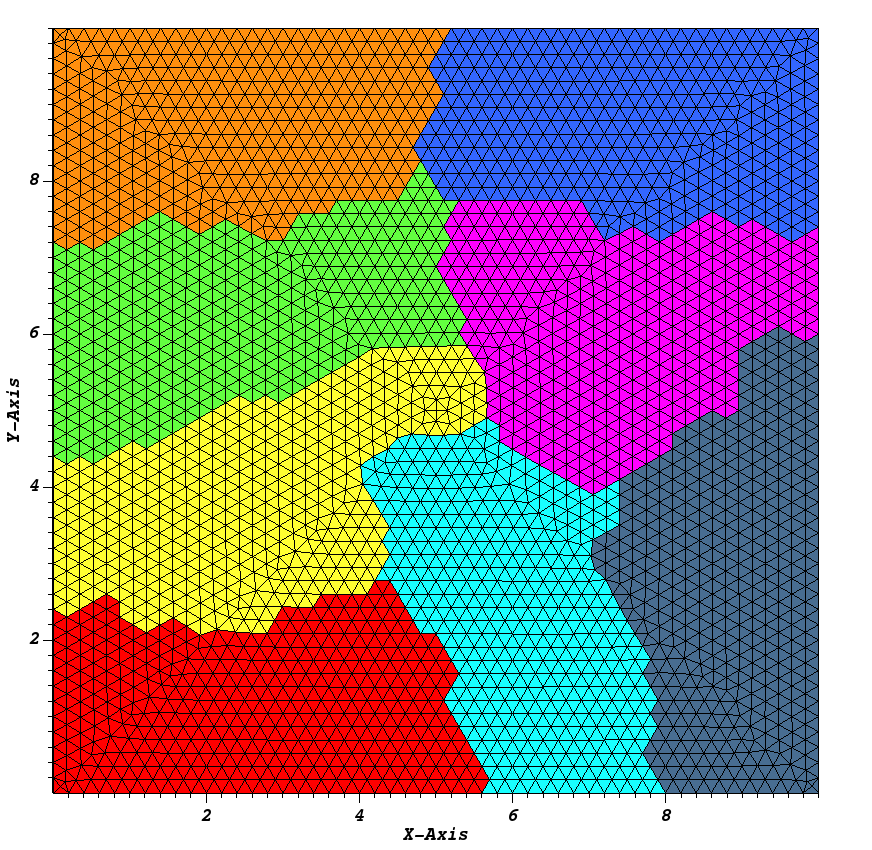
\includegraphics[width=.8\linewidth]{figures/metis_part_8.png}
		\caption{Exemple de partitionnement avec \textit{Metis} en utilisant 8 processus.}
		\label{fig:metis_part_8}
	\end{subfigure}    
	\hfill
	\begin{subfigure}{.45\textwidth}
		\centering
		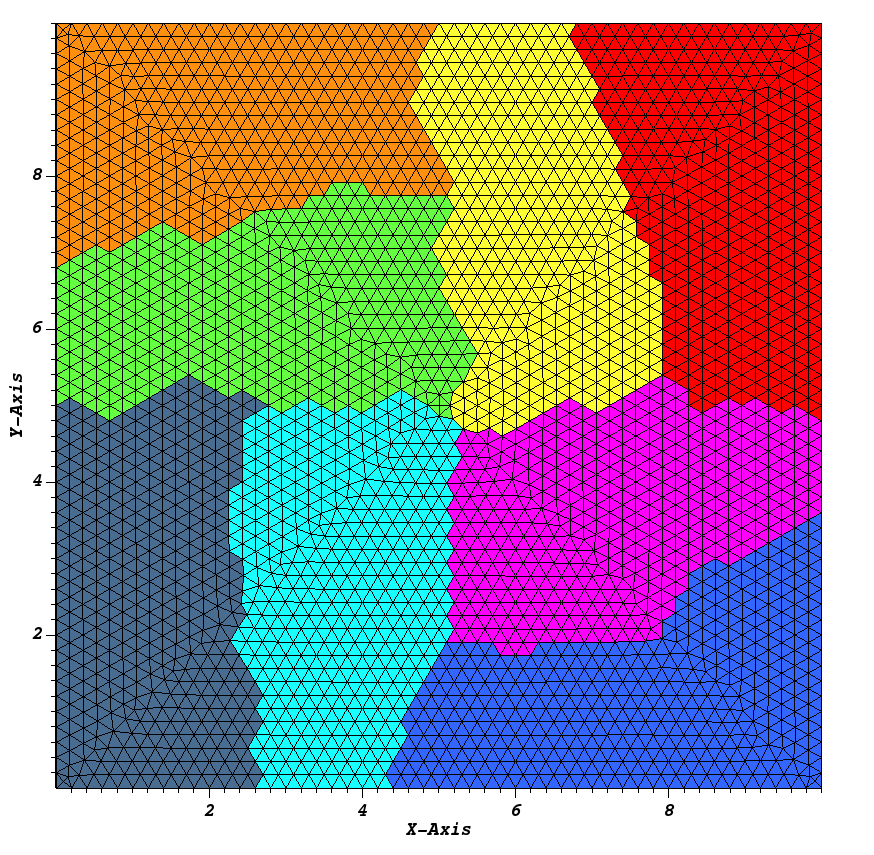
\includegraphics[width=.8\linewidth]{figures/scotch_part_8.png}
		\caption{Exemple de partitionnement avec \textit{Scotch} en utilisant 8 processus.}
		\label{fig:scotch_part_8}
	\end{subfigure}
	
	\caption{Différents partitionnement de maillages avec \textit{Metis} et \textit{Scotch}.}
	\label{fig:part_metis_scotch}
\end{figure}

\subsection{Éléments finis (EF)}
\noindent Afin de réaliser les différents speed-up avec le code Éléments Finis, il y a toute une partie de pré-traitement, entre le moment où on part du maillage, et le moment où on partitionne ce même maillage en sous-domaines pour résoudre notre problème. La figure \ref{fig:processus_generation} illustre ce traitement.

\begin{figure}[H]
	\centering
	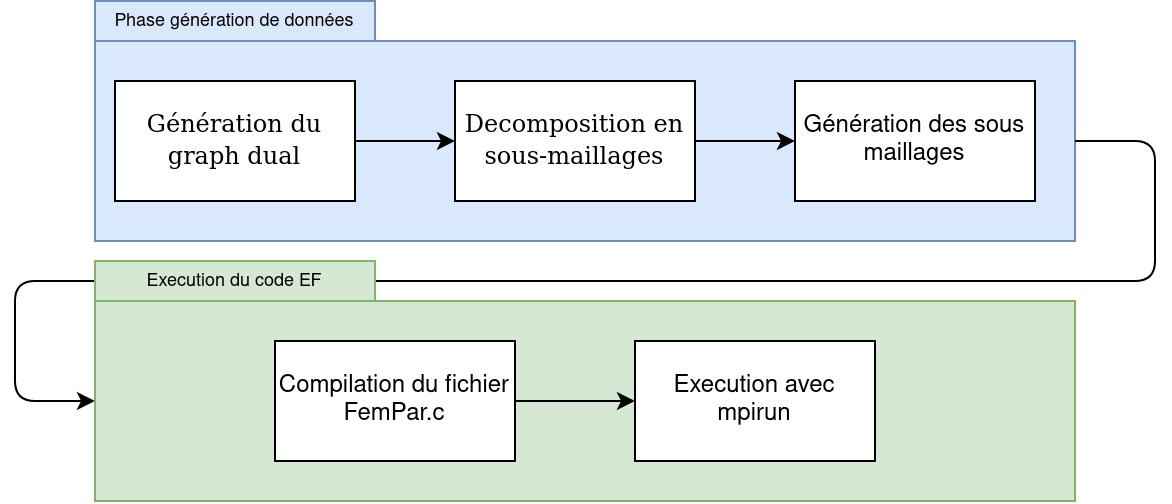
\includegraphics[width=0.70\linewidth]{figures/processus_experience_simulation.png}
	\caption{Processus de génération des sous-maillages et d'exécution du code EF.}
	\label{fig:processus_generation}
\end{figure}

\noindent Il a été rajouté dans le code EF un \textit{timer} mesurant les performances en temps du gradient conjugué, qui sera ensuite écrit dans un fichier, c'est de cette manière que nous allons pouvoir calculer le speed-up par la suite. 

\paragraph{Remarque :} lors de la partie découpage en sous-maillages, \textbf{Metis} génère une erreur si on essaie de le faire pour \textit{une} partition seulement ($k=1$), mais ce n'est pas le cas avec \textbf{Scotch}.


\subsection{Courbes et performances}

\begin{figure}[H]
	\centering
	\begin{subfigure}{.45\textwidth}
		\centering
		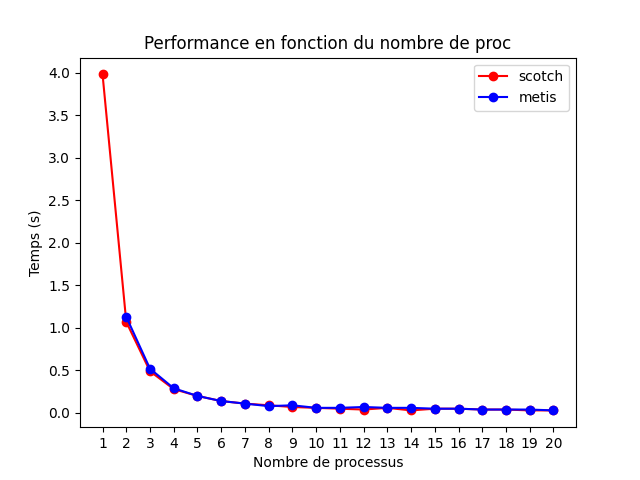
\includegraphics[width=\linewidth]{figures/perf_maillage_5000.png}
		\caption{Performances obtenues (en \textit{seconde}) sur \textit{plafrim} avec un maillage initiale de 5000 n\oe uds.}
		\label{fig:perf_maillage_5000}
	\end{subfigure}    
	\hfill
	\begin{subfigure}{.45\textwidth}
		\centering
		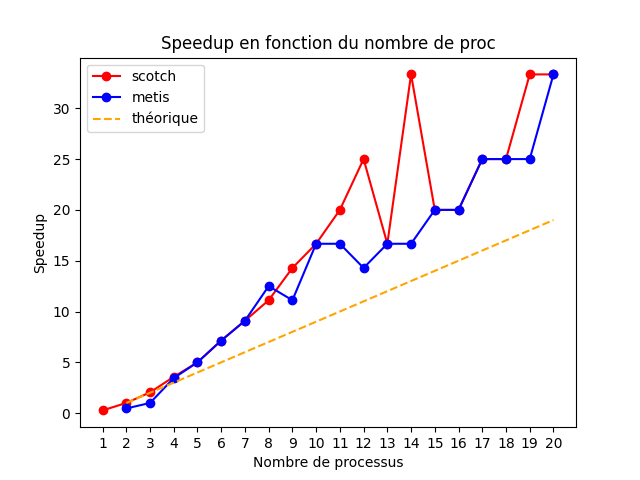
\includegraphics[width=\linewidth]{figures/speedup_maillage_5000.png}
		\caption{Speed-up obtenu pour un maillage de 5000 n\oe uds.}
		\label{fig:speed_up_maillage_5000}
	\end{subfigure}
	
	\caption{Courbes de performances et de speed-up avec un partitionnement Metis et Scotch.}
	\label{fig:perf_speed-up_maillage_5000}
\end{figure}

\noindent On remarque que sur la courbe de la figure \ref{fig:perf_maillage_5000}, le temps d'exécution diminue au fur et à mesure que l'on augmente le nombre de processus, ce qui est un comportement attendu. En revanche ce qui l'est moins, c'est que lorsqu'on calcule le speed-up\footnote{Calculé en fonction du temps et du nombre de processus, avec comme valeur de référence le temps pris sur \textbf{2} processus}, on se retrouve avec une valeur bien supérieure au speed-up théorique\footnote{Calculé par rapport au temps de référence; avec $N$ processus on est censé aller $N$ fois plus vite que le temps de référence (au plus)}. Ce qui peut expliquer cela, c'est le fait que le maillage de base soit si petit, et qu'on se retrouve avec la plupart des valeurs du calcul stockées dans le cache.

\noindent Nous avons donc testé sur un maillage bien plus grand (90000 n\oe uds), afin de voir si on retrouvait les mêmes observations que précédemment. 

%\paragraph{}
\noindent Les figures \ref{fig:perf_maillage_5000} et \ref{fig:perf_maillage_90000} ont la même allure, et le temps passé à calculer semble proportionnel au nombre de processus. Pour ce qui est du speed-up sur le maillage de taille 90000 (figure \ref{fig:perf_maillage_90000} et \ref{fig:speed_up_maillage_90000}), nous avons pris comme valeur de référence le temps d'exécution pour 4 processus (et non 1), afin d'obtenir des valeurs plus proches de la réalité. Il se trouve que nous observons le même phénomène que précédemment, ce qui est assez étrange vu la taille du problème en entrée du programme.

\begin{figure}[H]
	\centering
	\begin{subfigure}{.45\textwidth}
		\centering
		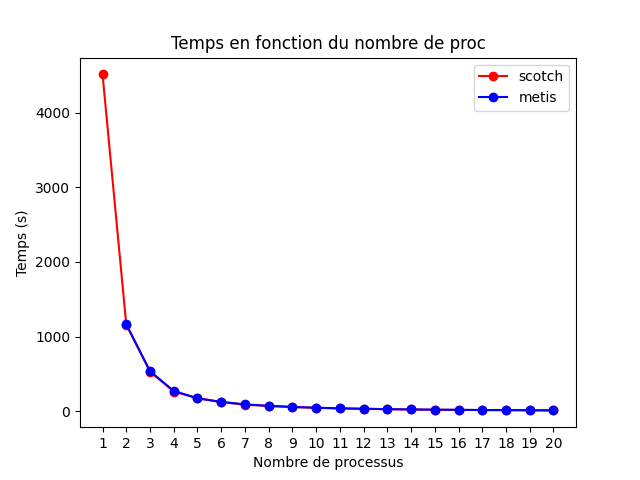
\includegraphics[width=.9\linewidth]{figures/temps_maillage_90000.png}
		\caption{Performances obtenues (en \textit{seconde}) sur \textit{plafrim} avec un maillage initial de 90000 n\oe uds.}
		\label{fig:perf_maillage_90000}
	\end{subfigure}    
	\hfill
	\begin{subfigure}{.45\textwidth}
		\centering
		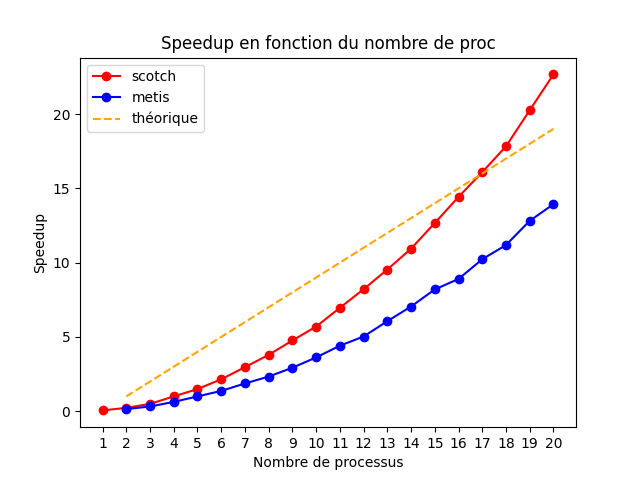
\includegraphics[width=.9\linewidth]{figures/speedup_maillage_90000.png}
		\caption{Speedup obtenu pour un maillage de 90000 n\oe uds.}
		\label{fig:speed_up_maillage_90000}
	\end{subfigure}
	
	\caption{Courbes de performances et de speed-up avec un partitionnement Metis et Scotch}
	\label{fig:perf_speedup_maillage_90000}
\end{figure}

\paragraph{Parallélisme} En ce qui concerne le parallélisme effectué dans le code, il se situe au niveau de la fonction \texttt{InnerProduct()}, où chaque processus va faire son produit scalaire localement, pour ensuite faire une réduction sur toutes les partitions et les sommer. Également, la fonction \texttt{Update()} comprend des directives MPI, pour l'envoi et la réception des données partagées avec les processeurs voisins, ce qui se traduit par des directives \texttt{MPI\_Isend()} et \texttt{MPI\_Irecv()} afin de ne bloquer ni l'envoi, ni la réception de données.


\paragraph{Environnement} Pour ce qui est de l'environnement de calcul utilisé, nous avons utilisé Plafrim, plus précisément les n\oe uds mistral, en se mettant seul sur un n\oe ud à chaque fois (option \texttt{{-}{-}exclusive}) sur un nombre de c\oe urs variant de 1 à 20.


\section{Décomposition de domaine de Schwarz sur maillage cartésien}

\noindent Dans cette partie nous étudierons la mise en \oe uvre de l'algorithme de Schwarz additif pour une équation bien connue et facile à discrétiser : l'équation de Poisson. Il est important de souligner que toutes les remarques que nous ferons dans la suite sont propres à ce problème et à la taille du stencil pour obtenir une erreur d'ordre 2 : il est facile de remarquer que le problème est tout autre lorsque nous avons des stencils plus grands (ne serait-ce que pour obtenir de l'ordre 4 pour le même problème). 

\subsection{Domaine de calcul et équation}
\noindent À l'origine nous devions étudier l'équation de la chaleur, mais comme la seule différence par rapport au problème de Poisson réside dans l'ajout d'une boucle temporelle, nous avons décidé de nous concentrer uniquement sur le cas stationnaire
\begin{tcolorbox}[colback=MyRed!5!white,colframe=MyRed,halign=left,leftrule=3mm, rightrule=0mm, toprule=0mm, bottomrule=0mm]
	\begin{equation}
		\begin{cases}
			-\Delta u = f & \text{ dans $\Omega$}\\
			u = g & \text{ sur $\partial \Omega$}
		\end{cases},\label{eq:poisson}
	\end{equation}
	pour un ouvert $\Omega$ de $\mathbb{R}^2$ et $f$, $g$ deux fonctions de $\Omega \to \mathbb{R}$.
\end{tcolorbox}
 \noindent La condition de Dirichlet sur le bord de $\Omega$ pourrait être aisément remplacée par une condition de Neumann sur une partie de ce bord et nous aurions toujours un problème bien posé. Ce cas n'est pas étudié ici, mais est très simple à mettre en \oe uvre pour un stencil de taille 5 sur un carré. Concernant $\Omega$ lui-même nous avons choisi un domaine carré, de préférence $\left[0, 1\right] x \left[0, 1\right]$ pour mener nos simulations car c'est un domaine qui se prête à la discrétisation en maillage structuré.\\

\noindent Deux problèmes seront résolus par la suite
\begin{tcolorbox}[colback=MyRed!5!white,colframe=MyRed,halign=left,leftrule=3mm, rightrule=0mm, toprule=0mm, bottomrule=0mm]
	\begin{equation}
		f_1(x, y) = 2 x (1-x) + 2y(1-y) \hspace{1cm}\text{ et }\hspace{1cm} g_1 \equiv 0 \label{eq:problem1}\tag{$\star$}
	\end{equation}
	de solution analytique $u_1(x, y) = xy(1-x)(1-y)$
\end{tcolorbox}
\noindent et 
\begin{tcolorbox}[colback=MyRed!5!white,colframe=MyRed,halign=left,leftrule=3mm, rightrule=0mm, toprule=0mm, bottomrule=0mm]
	\begin{equation}
	f_2(x, y) = \sin\left(x\right) + \cos\left(y\right) \hspace{1cm}\text{ et }\hspace{1cm} g_2 = f_2 \label{eq:problem2}\tag{$\star\star$}
	\end{equation}
	de solution analytique $ u_2 = - f_2$.
\end{tcolorbox}

\subsection{Décomposition de domaine Schwarz additif}
\subsubsection{Décomposition de domaine}
\noindent La décomposition de domaine consiste à partitionner le domaine de calcul $\Omega$ en plusieurs morceaux, les \textit{partitions}. Le but est d'équirépartir le nombre de degrés de liberté entre chaque domaine nouvellement créé, ainsi que de résoudre en \textit{parallèle} le même problème avec des tailles moindres par rapport au domaine de calcul initial. Ces résolutions sont alors découplées et peuvent s'effectuer \textit{en même temps}. C'est ici que le calcul parallèle prend tout son sens.\\

\noindent Un seul défaut demeure pourtant : il faut \textbf{harmoniser} les valeurs entre les partitions puisqu'à l'échelle du domaine entier, un degré de liberté ne peut avoir qu'une seule valeur et la réunion des différentes solutions trouvées doit correspondre à l'unique solution valable sur le domaine $\Omega$ tout entier (le problème initial étant bien posé).\\
\begin{figure}[H]
	\incfig{0.47}{ddomega}
	\incfig{0.47}{dd}
	\caption{Exemple de décomposition avec recouvrement d'un domaine $\Omega$ quelconque.}
	\label{fig:dd}
\end{figure}
\noindent La décomposition de domaine avec recouvrement apporte une solution à cet enjeu. Le but est de partitionner le domaine en créant des zones de recouvrement plus ou moins grandes appartenant à au moins 2 partitions. Ces zones de recouvrement, dont la taille est en pratique variable, constituent le c\oe ur même de cette \textbf{harmonisation}. Elles sont des zones d'échanges de valeurs entre partitions et permettent une transmission, une sorte de liaison de continuité, entre deux domaines. Il va sans dire que la résolution du problème à l'échelle du domaine initial $\Omega$ ne peut pas se faire en une seule fois.\\

\noindent Si notre domaine est partitionné en deux zones $D_1$ et $D_2$, comme dans la figure \ref{fig:dd}, la zone d'échanges doit avertir $D_1$ des valeurs calculées sur $D_2$ et inversement. Un procédé itératif se dégage alors, le but étant d'atteindre un état \textit{stationnaire} de sorte que les valeurs reçues par $D_1$ sur $D_2$ ne \textit{modifient plus} les valeurs des degrés de libertés de $D_2$ (et inversement). Nous venons de dégager un critère de \textit{convergence}.\\

\subsubsection{La méthode de Schwarz additif}
\noindent La méthode de Schwarz additif (il existe d'autres méthodes qui ne seront pas développées ici) est la mécanique de la zone d'échange. C'est une méthode itérative dans le sens où elle demande de résoudre  plusieurs fois l'équation sur chaque partition et d'échanger des valeurs. Elle est basée sur l'échange de conditions aux bords que nous qualifierons de \textbf{conditions aux bords virtuels}\footnote{bords entre entre deux partitions en incluant la zone de recouvrement.}.\\
Plusieurs conditions aux bords peuvent être envoyées, la plus évidente étant celle de type Dirichlet. Si nous reprenons notre figure \ref{fig:dd} et que nous notons le recouvrement $R = D_1 \cap D_2$, alors nous nous ramenons aux deux problèmes suivants\vspace{5mm}\\
\begin{minipage}{0.47\textwidth}
	\begin{equation}
		\begin{cases}
		-\Delta u_{[1]} = f_{[1]}&\text{ dans $D_1$}\\
		u_{[1]} = g & \text{ sur $\partial \Omega \cap \partial D_1$}\\
		u_{[1]} = u_{[2]} &\text{ sur $\Gamma_1 := \partial R \cap D_2$}
		\end{cases}\label{eq:d1}
	\end{equation}
\end{minipage}
\hfill
\begin{minipage}{0.47\textwidth}
	\begin{equation}
	\begin{cases}
	-\Delta u_{[2]} = f_{[2]}&\text{ dans $D_2$}\\
	u_{[2]} = g & \text{ sur $\partial \Omega \cap \partial D_2$}\\
	u_{[2]} = u_{[1]} &\text{ sur $\Gamma_2 := \partial R \cap D_1$}
	\end{cases}
	\end{equation}
\end{minipage}
\vspace{2cm}\\
\noindent Nous obtenons un algorithme naïf de résolution\vspace{3mm}\\
\begin{minipage}{0.47\textwidth}
\begin{algorithm}[H]
		\SetAlgoLined
		$u_{[2], \Gamma_1} = 0$\;
		Calculer $u_{[1], \partial\Omega}$\;
		\While{critère}{
			Imposer $u_{[1], \partial\Omega}$ et $u_{[2], \Gamma_1}$ \;
			Résoudre $-\Delta u_{[1]} = f_{[1]}$\;
			Envoyer à $\boxed{2}$ $u_{[1], \Gamma_2}$\;
			Recevoir de $\boxed{2}$ $u_{[2], \Gamma_1}$\;
	}
\caption{Schwarz additif sur $D_1$}
\end{algorithm}
\end{minipage}\hfill
\begin{minipage}{0.47\textwidth}
	\begin{algorithm}[H]
		\SetAlgoLined
		$u_{[1], \Gamma_2} = 0$\;
		Calculer $u_{[2], \partial\Omega}$\;
		\While{critère}{
			Imposer $u_{[2], \partial\Omega}$ et $u_{[1], \Gamma_2}$ \;
			Résoudre $-\Delta u_{[2]} = f_{[2]}$\;
			Envoyer à $\boxed{1}$ $u_{[2], \Gamma_1}$\;
			Recevoir de $\boxed{1}$ $u_{[1], \Gamma_2}$\;
		}
\caption*{Schwarz additif sur $D_2$}
	\end{algorithm}
\end{minipage}
\vspace{3mm}\\
\noindent Une illustration de la méthode est donné en suivant
\begin{figure}[H]
	\incfig{0.5}{dditer}
	\caption{Principe des itérations de la méthode de Schwarz additif en 1D (conditions de Dirichlet).}
\end{figure}
\noindent Échanger des conditions de Dirichlet fonctionne pour notre problème \eqref{eq:poisson} mais nous pouvons remarquer qu'il est indépendant de l'équation résolue. Ce type de conditions aux bords fonctionnerait pour n'importe quelles équations.\\

\subsubsection{Condition de type Robin}
\paragraph{Théorie}
\noindent Regardons donc avec un peu plus de finesse ce qu'il se passe sur un bord virtuel $\Gamma \subset \Omega$ (certains préféreront sans doute employer ici la notion d'interface qui est assez parlante). Nous définissons $D_1$ et $D_2$ comme une partition de $\Omega$ au sens mathématique du terme, ie $\partial D_1 \cap \partial D_2 := \Gamma$. \\
Nous considérons ici \eqref{eq:poisson} après relèvement (ie $u = 0$ sur $\partial \Omega$). Soit $\varphi \in \mathcal{C}^{\infty}_c\left[\Omega\right]$ une distribution sur $\Omega$, la formulation variationnelle est
\begin{equation*}
	-\left<\Delta u\mid \varphi\right>_{\Omega} = \left<f\mid \varphi\right>_{\Omega}
\end{equation*}
En notant $u_{[1]} := u$ sur $D_1$ et $u_{[2]} := u$ sur $D_2$, alors
\begin{equation*}
	\Longrightarrow -\left<\Delta u_{[1]}\mid \varphi\right>_{D_1} - \left<\Delta u_{[2]}\mid \varphi\right>_{D_2} = \left<f\mid \varphi\right>_{\Omega}
\end{equation*}
En appliquant les formules de Green
\begin{equation*}
	\left<\Delta u\mid \varphi\right>_{\Omega} = \left<\nabla u \cdot n\mid \varphi\right>_{\partial\Omega} - \left<\nabla u\mid \nabla\varphi\right>_{\Omega}\hspace{1cm}\text{ et }\hspace{1cm}
	\left<\nabla u\mid \nabla\varphi\right>_{\Omega} = \left<u\mid \nabla\varphi \cdot n\right>_{\partial\Omega}-\left<u\mid \Delta\varphi\right>_{\Omega},
\end{equation*}
nous obtenons
\begin{align*}
	\Longrightarrow &-\left<\nabla u_{[1]}\cdot n_{D_1}\mid \varphi\right>_{\partial D_1} + \left<u_{[1]}\mid\nabla \varphi\cdot n_{D_1}\right>_{\partial D_1} - \left<u_{[1]} \mid \Delta \varphi\right>_{D_1}\\
	\hspace{1cm} &-\left<\nabla u_{[2]}\cdot n_{D_2}\mid \varphi\right>_{\partial D_2} + \left<u_{[2]}\mid\nabla \varphi\cdot n_{D_2}\right>_{\partial D_2} - \left<u_{[2]} \mid \Delta \varphi\right>_{D_2} = \left<f\mid \varphi\right>_{\Omega}
\end{align*}
et comme $\varphi \equiv 0$ sur $\partial\Omega$ et en posant $n:= n_{D_1} = -n_{D_2}$ sur $\Gamma$ alors
\begin{equation*}
\Longrightarrow -\left<\left(\nabla u_{[1]}-\nabla u_{[2]}\right)\cdot n\mid \varphi\right>_{\Gamma} + \left<u_{[1]} - u_{[2]}\mid\nabla \varphi\cdot n\right>_{\Gamma} - \left<u_{[1]} \mid \Delta \varphi\right>_{D_1} - \left<u_{[2]} \mid \Delta \varphi\right>_{D_2} = \left<f\mid \varphi\right>_{\Omega}
\end{equation*}
Par définition du partitionnement nous souhaitons que 
\begin{equation*}
\left< u \mid \Delta \varphi\right>_{\Omega} = \left< u_{[1]} \mid \Delta \varphi\right>_{D_1} + \left< u_{[2]} \mid \Delta \varphi\right>_{D_2}
\end{equation*}
(rappelons qu'ici il n'y a pas de recouvrement), donc si nous réappliquons deux fois les formules de Green sur $\Omega$ tout entier, alors
\begin{equation*}
\left<-\left(\nabla_n u_{[1]}-\nabla_n u_{[2]}\right) \mid \varphi\right>_{\Gamma} + \left<u_{[1]} - u_{[2]}\mid\nabla_n \varphi\right>_{\Gamma} = \left<\Delta u + f\mid \varphi\right>_{\Omega} \overset{\text{équation }\eqref{eq:poisson}}{=} 0
\end{equation*}
En notant $[\kappa] := \kappa_{[2]}- \kappa_{[1]}$ le saut à l'interface pour une quantité $\kappa$, l'égalité précédente est exactement
\begin{equation*}
\left< [\nabla_n u] \mid \varphi\right>_{\Gamma} - \left<[u]\mid\nabla \varphi\cdot n\right>_{\Gamma} = 0
\end{equation*}
Nous pouvons remarquer que  si nous imposons un saut nul sur $u$ et son gradient normal, ie $[u] = 0$ et $ [\nabla_n u] = 0$, alors $\alpha [\nabla_n u] - \beta[u] = 0$, c'est-à-dire
\begin{equation*}
\alpha \nabla_n u_{[1]} + \beta u_{[1]} = \alpha \nabla_n u_{[2]} + \beta u_{[2]}
\end{equation*}
Cette relation constitue une condition de bord virtuel dite de Robin.\\

\noindent Il est important de noter à ce stade qu'une condition de bord virtuel de type Dirichlet nécessite un recouvrement et non un simple partage de bord. En effet, imaginons que nos partitions $D_1$ et $D_2$ sont telles que $D_1 \cap D_2 = \Gamma$ soit un hyperplan de $\Omega$ (donc de mesure nulle avec la mesure sur $\Omega$). Alors \eqref{eq:d1} devient 
\begin{equation*}
	\begin{cases}
		-\Delta u_{[1]} = f_{[1]}&\text{ dans $D_1$}\\
		u_{[1]} = g & \text{ sur $\partial \Omega \cap \partial D_1$}\\
		u_{[1]} = u_{[2]} \equiv u_{[1]}  &\text{ sur $\Gamma$}
	\end{cases}
\end{equation*}
et nous pouvons remarquer que la condition de bord $u_{[1]}$ n'est plus mis-à-jour.

\paragraph{Discrétisation d'une condition de type Robin}
A contrario, une condition de type Robin ne semble pas demander une telle considération. Cela vient sans douter, de la façon qu'on peut imaginer imposer une condition de type Robin. Regardons donc la façon de discrétiser cette condition.
Soit $n = \left[n_x, n_y\right]$ la normale sortante à $D_1$ sur le bord virtuel $\Gamma$, et $g$ la valeur à imposer. Alors la condition de Robin est
\begin{equation}
	\alpha\nabla_n u + \beta u = g \hspace{2cm} \alpha, \beta \in \mathbb{R}.
\end{equation}
Nous considérons ici l'exemple d'un bord virtuel \textit{aligné} avec la grille de discrétisation, dans le code un bord non aligné avec la grille aura dans ses coins des conditions de type Dirichlet par défaut pour typiquement éviter les doubles conditions en un point :
\begin{equation*}
	\alpha n_x \partial_x u + \beta u = g_1 \hspace{1cm} \alpha n_y \partial_y u + \beta u = g_2
\end{equation*}
Nous rappelons que nous avons discrétisé l'équation avec un stencil de 5 points pour obtenir une erreur d'ordre 2. Il nous faut alors discrétiser la condition au bord avec le même ordre : nous utiliserons donc un schéma centré. Nous notons $u_{G}$ le "ghost" point, $u_{NG}$ le point "not-ghost" et $u_H$ est le point où nous voulons imposer la condition $g_H$
\begin{equation*}
	\alpha\frac{u_{G} - u_{NG}}{2d} + \beta u_H = g_H \hspace{1cm}\Longleftrightarrow \hspace{1cm} u_G = u_{NG}-\frac{2d\beta}{\alpha}u_H + \frac{2d}{\alpha}g_H
\end{equation*}

\subsection{Le recouvrement en pratique}
\subsubsection{Les différentes techniques de partitionnement}
\noindent Nous partons d'un domaine carré, précédemment maillé (en pratique le code nécessite un format de maillage ".lyra" généré par l'exécutable \textbf{generator-lyra}). Plusieurs techniques de partitionnement sont alors possibles en plus de la condition aux bords virtuels souhaité. Nous faisons appel à deux bibliothèque bien connues des partitionneurs : Metis \footnote{Metis : \url{http://glaros.dtc.umn.edu/gkhome/metis/metis/overview}} et Scotch \footnote{Scotch : \url{https://www.labri.fr/perso/pelegrin/scotch/}}. Nous avons implémenté quatre autres méthodes : en colonnes, en lignes, en damier et par équilibrage de diagramme de Voronoï.
\begin{figure}[H]
	\centering
	\begin{subfigure}[b]{0.45\textwidth}
		\hspace{-2.5cm}
		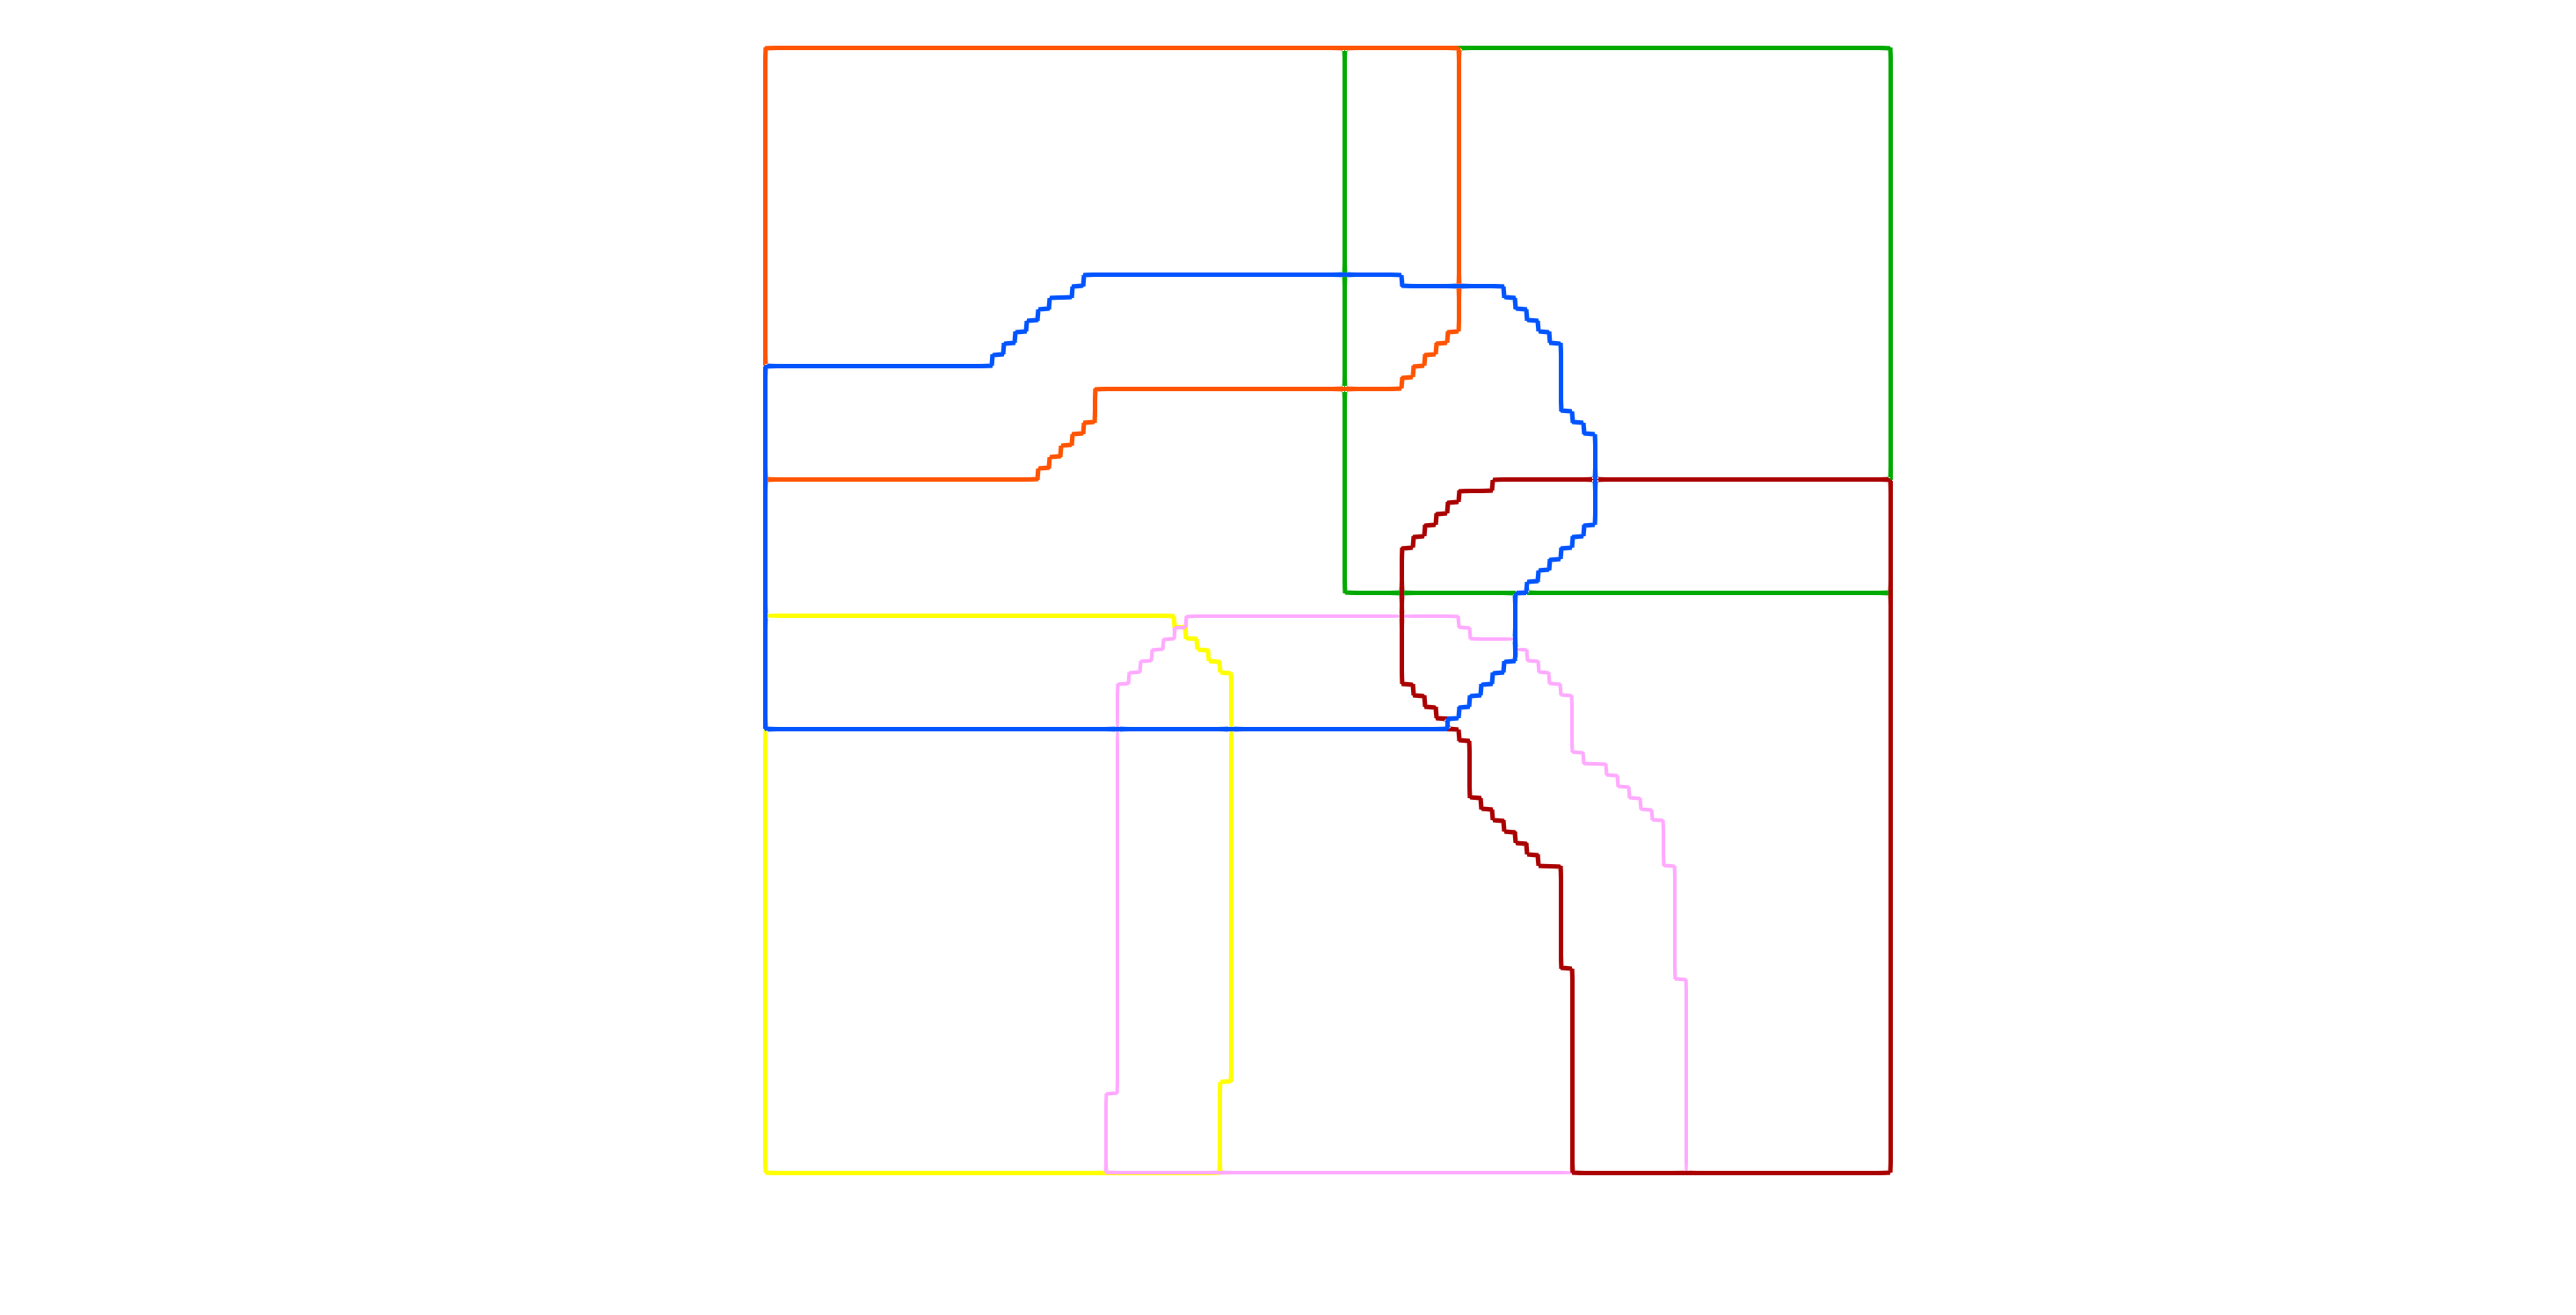
\includegraphics[width=1.5\textwidth]{metis_6.png}
		\caption{Metis}
	\end{subfigure}
\hfill
	\begin{subfigure}[b]{0.45\textwidth}
		\hspace{-2.5cm}
		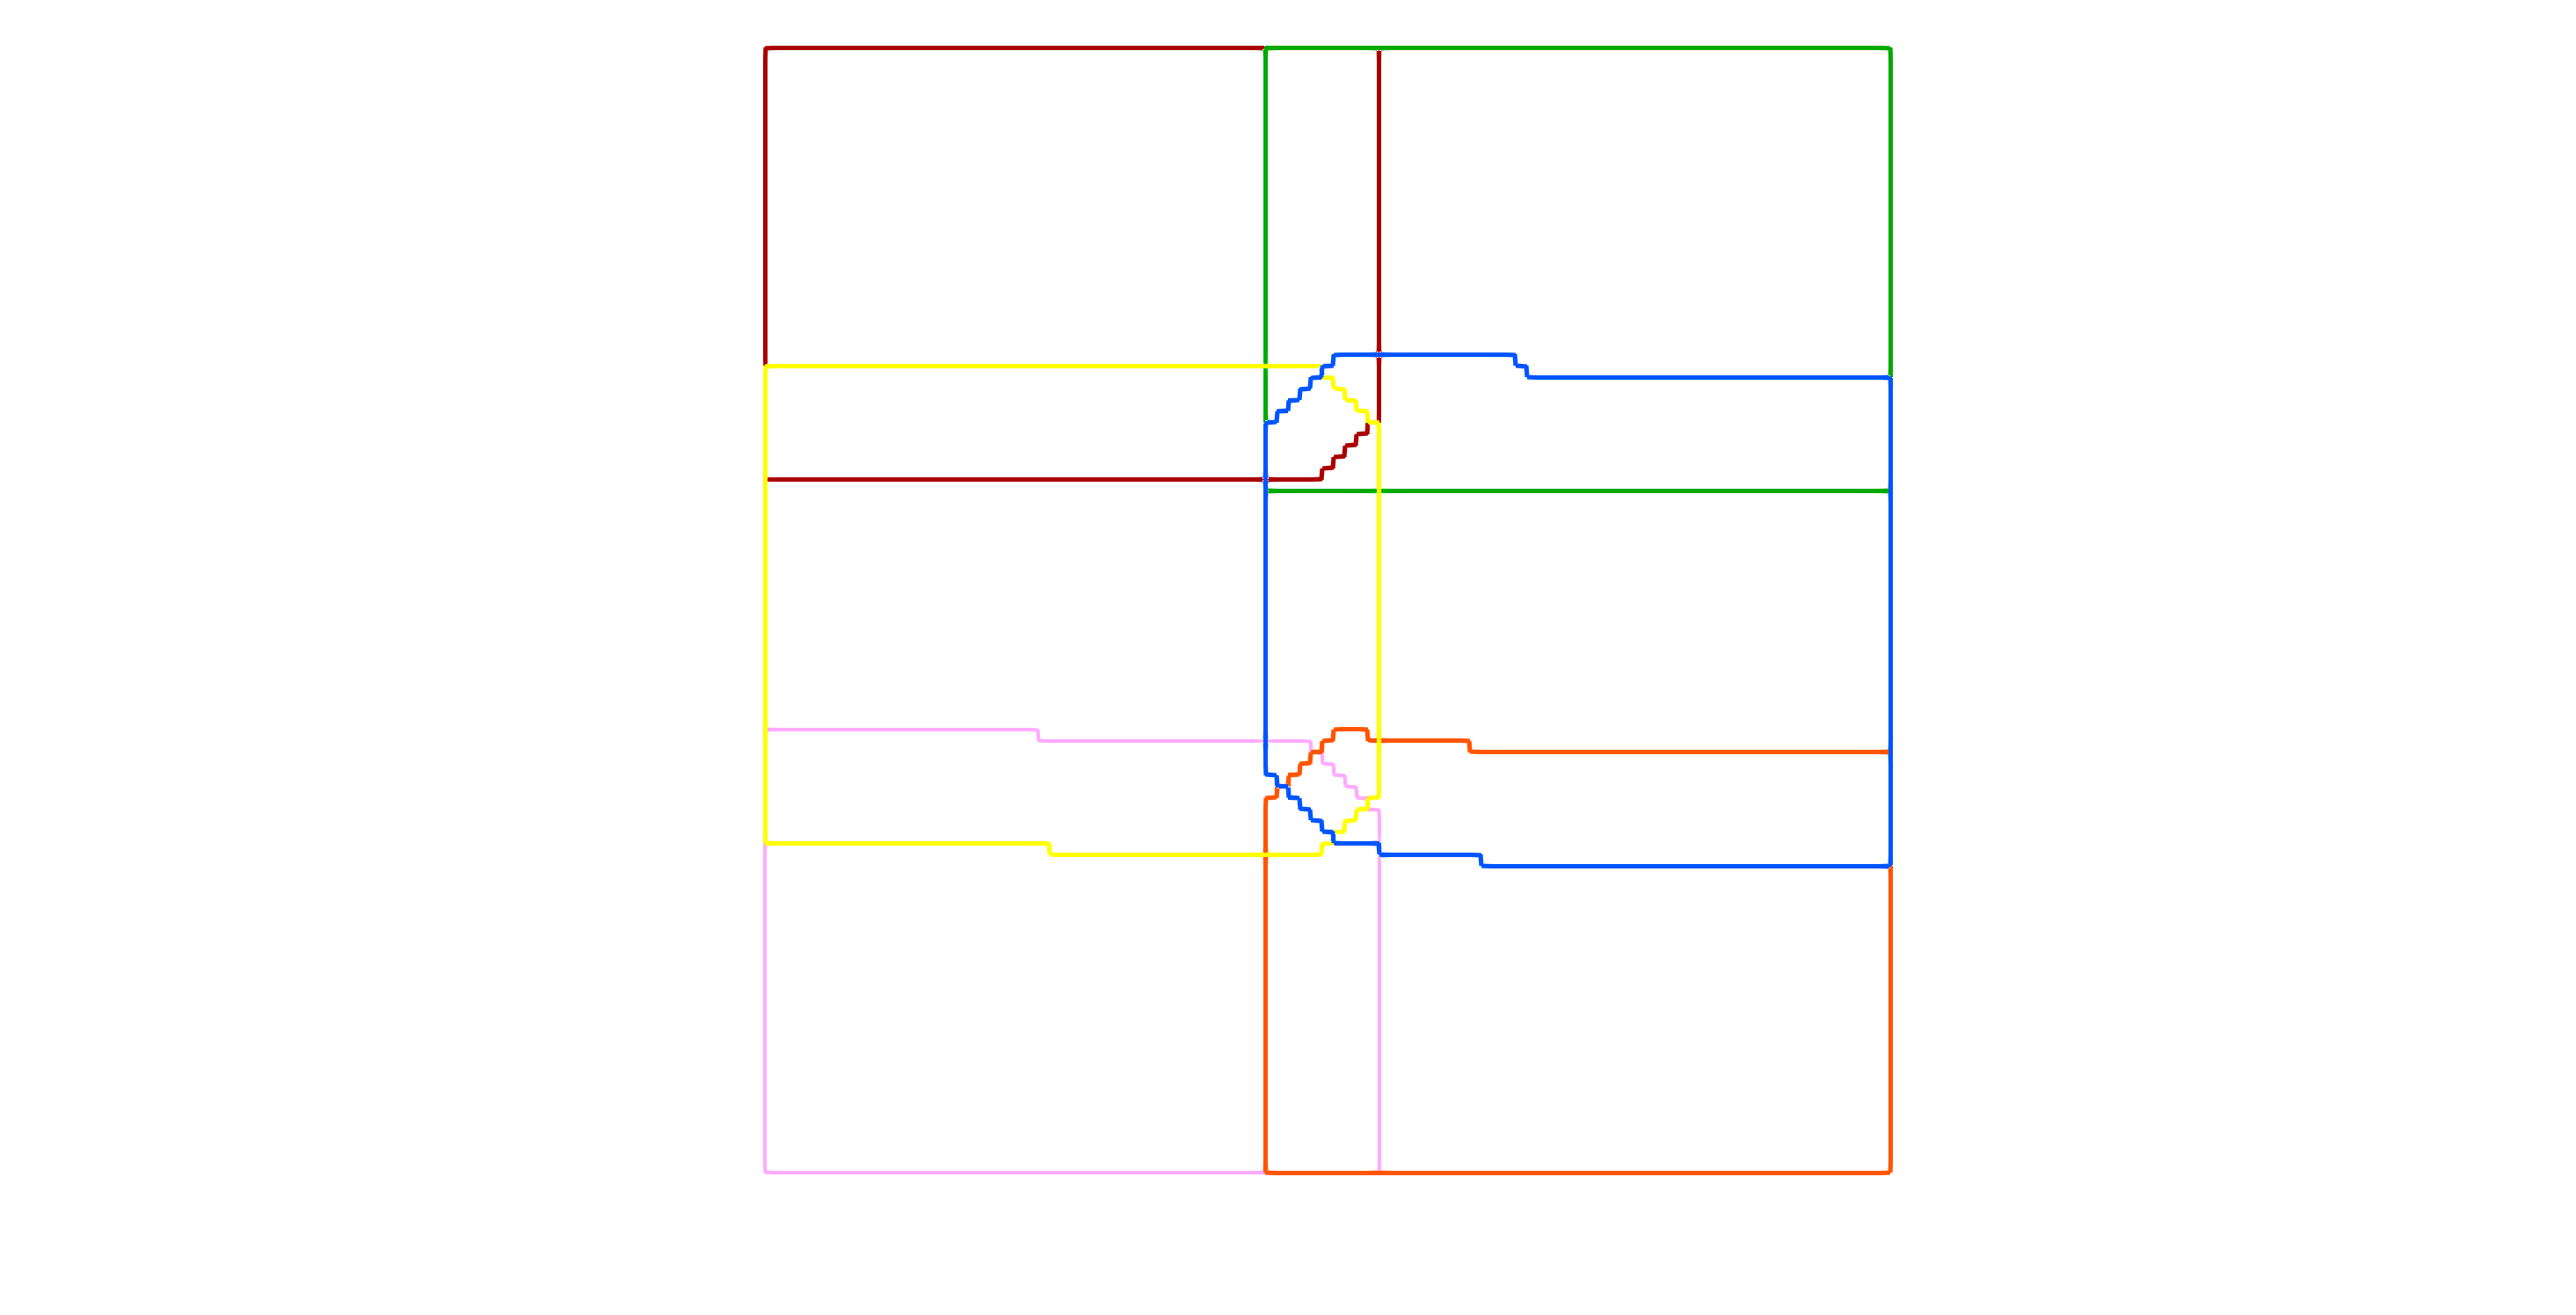
\includegraphics[width=1.5\textwidth]{scotch_6.png}
		\caption{Scotch}
	\end{subfigure}
\end{figure}
\begin{figure}[H]\ContinuedFloat
	\begin{subfigure}[b]{0.45\textwidth}
		\hspace{-2.5cm}
		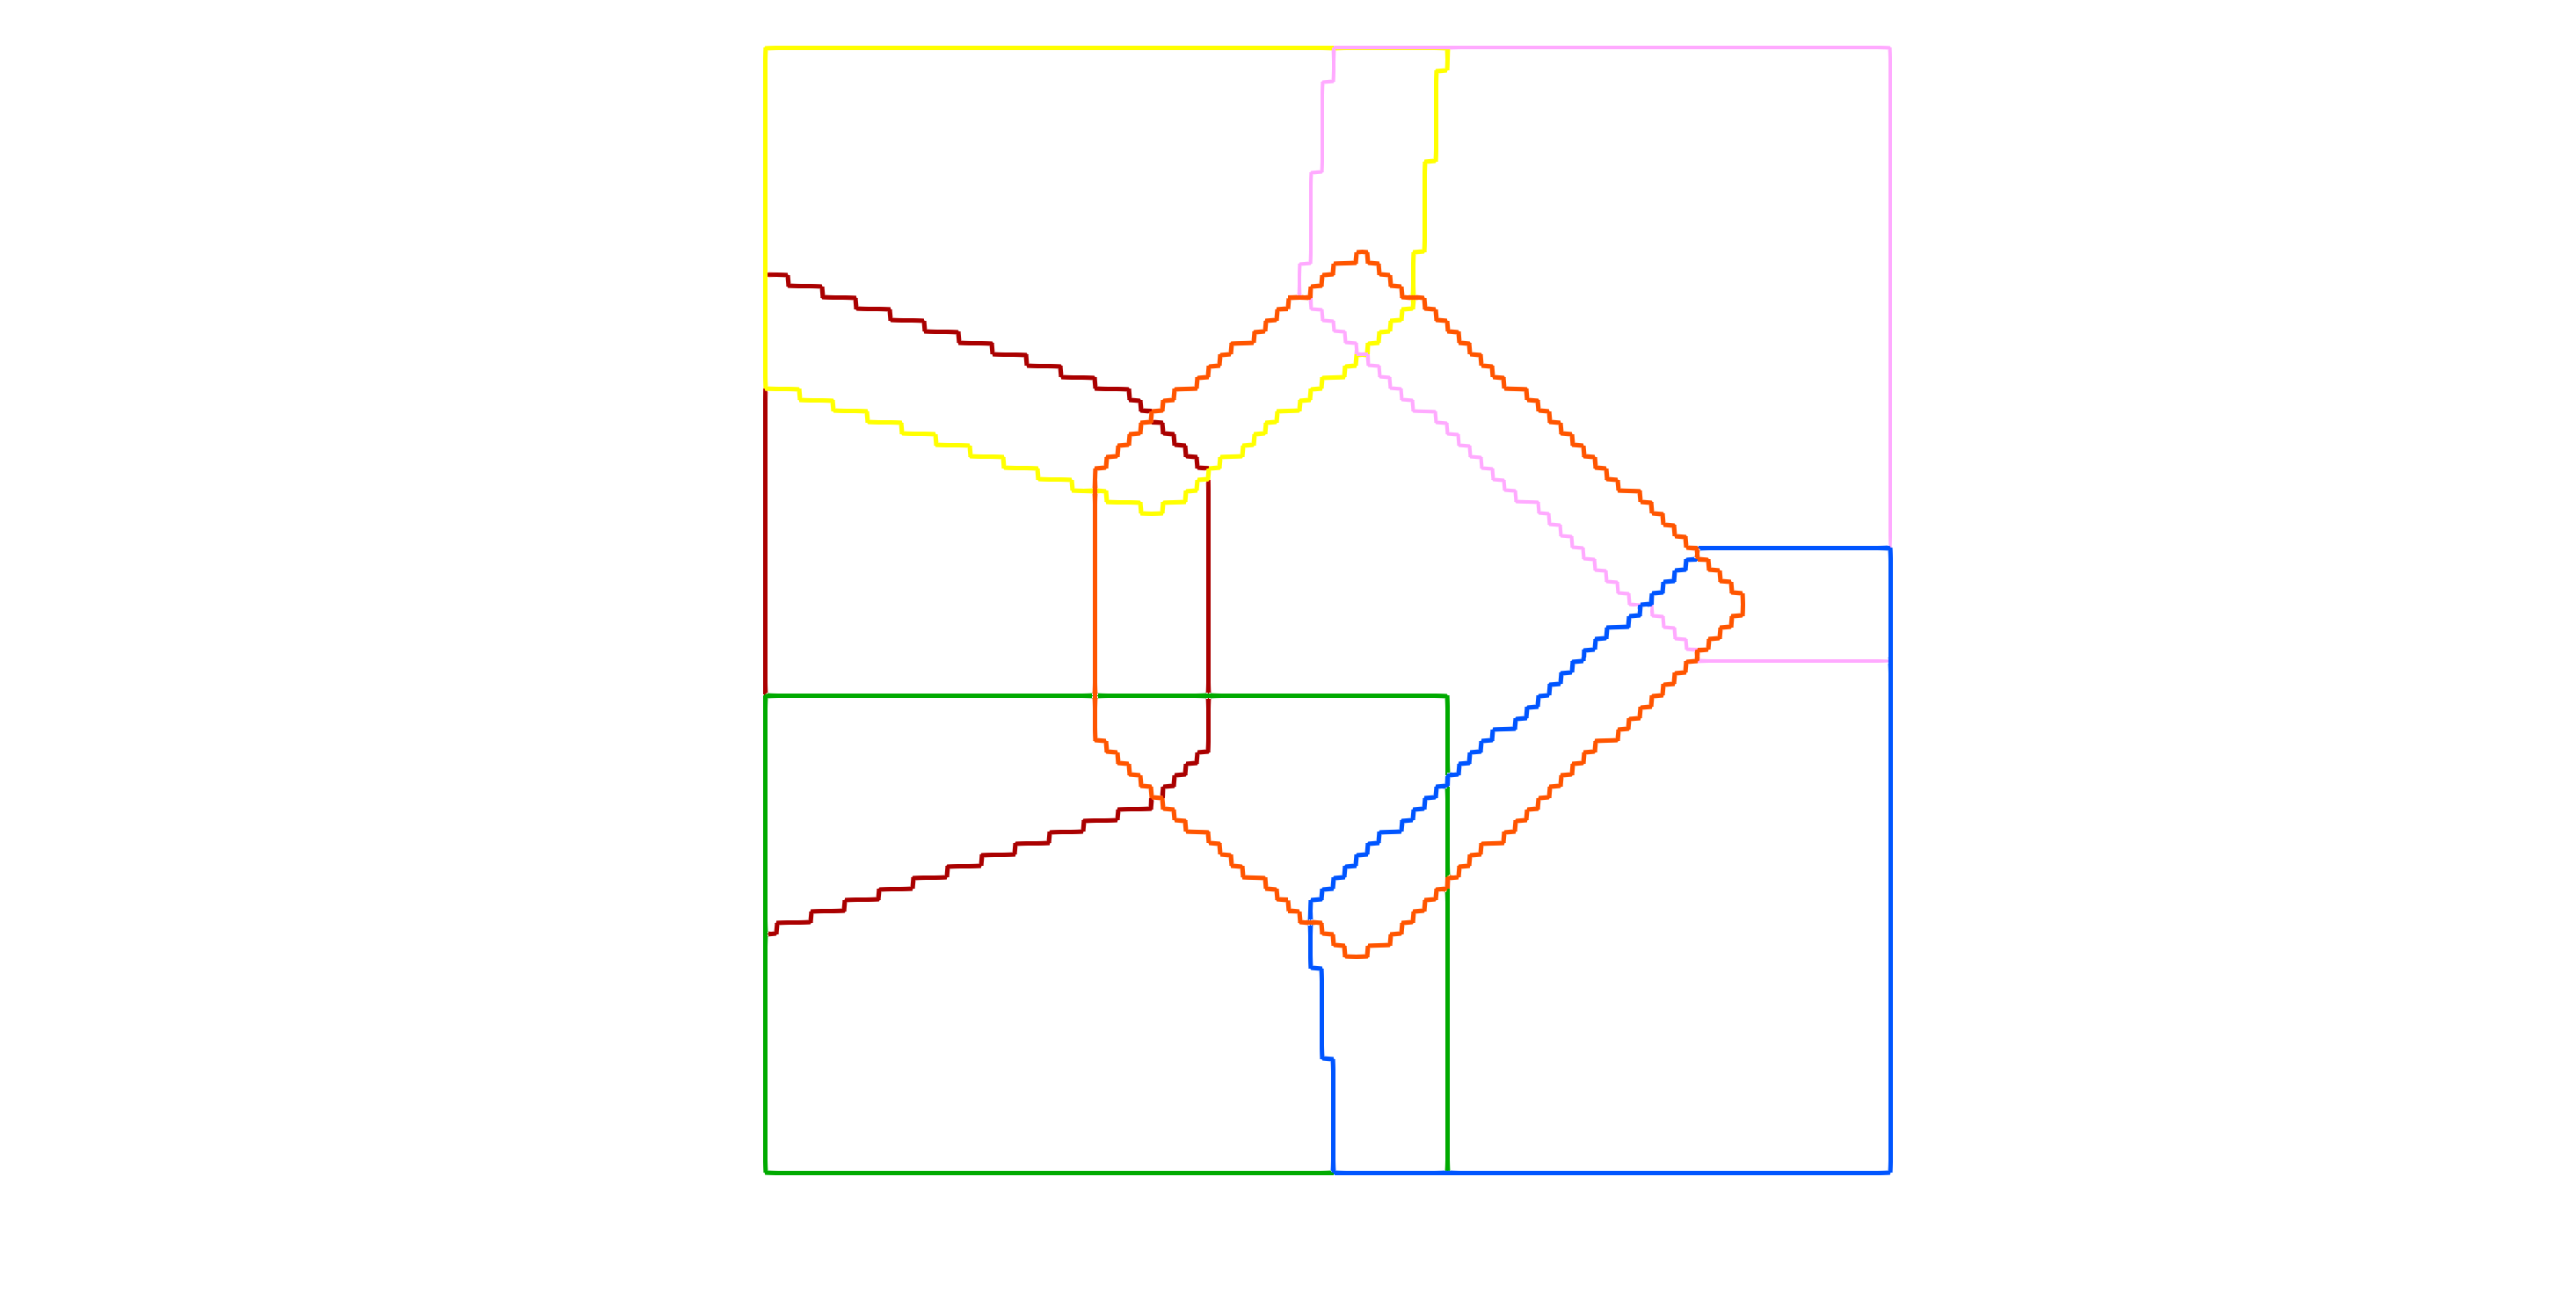
\includegraphics[width=1.5\textwidth]{voronoi_6.png}
		\caption{Voronoï}
	\end{subfigure}
	\hfill
	\begin{subfigure}[b]{0.45\textwidth}
		\hspace{-2.5cm}
		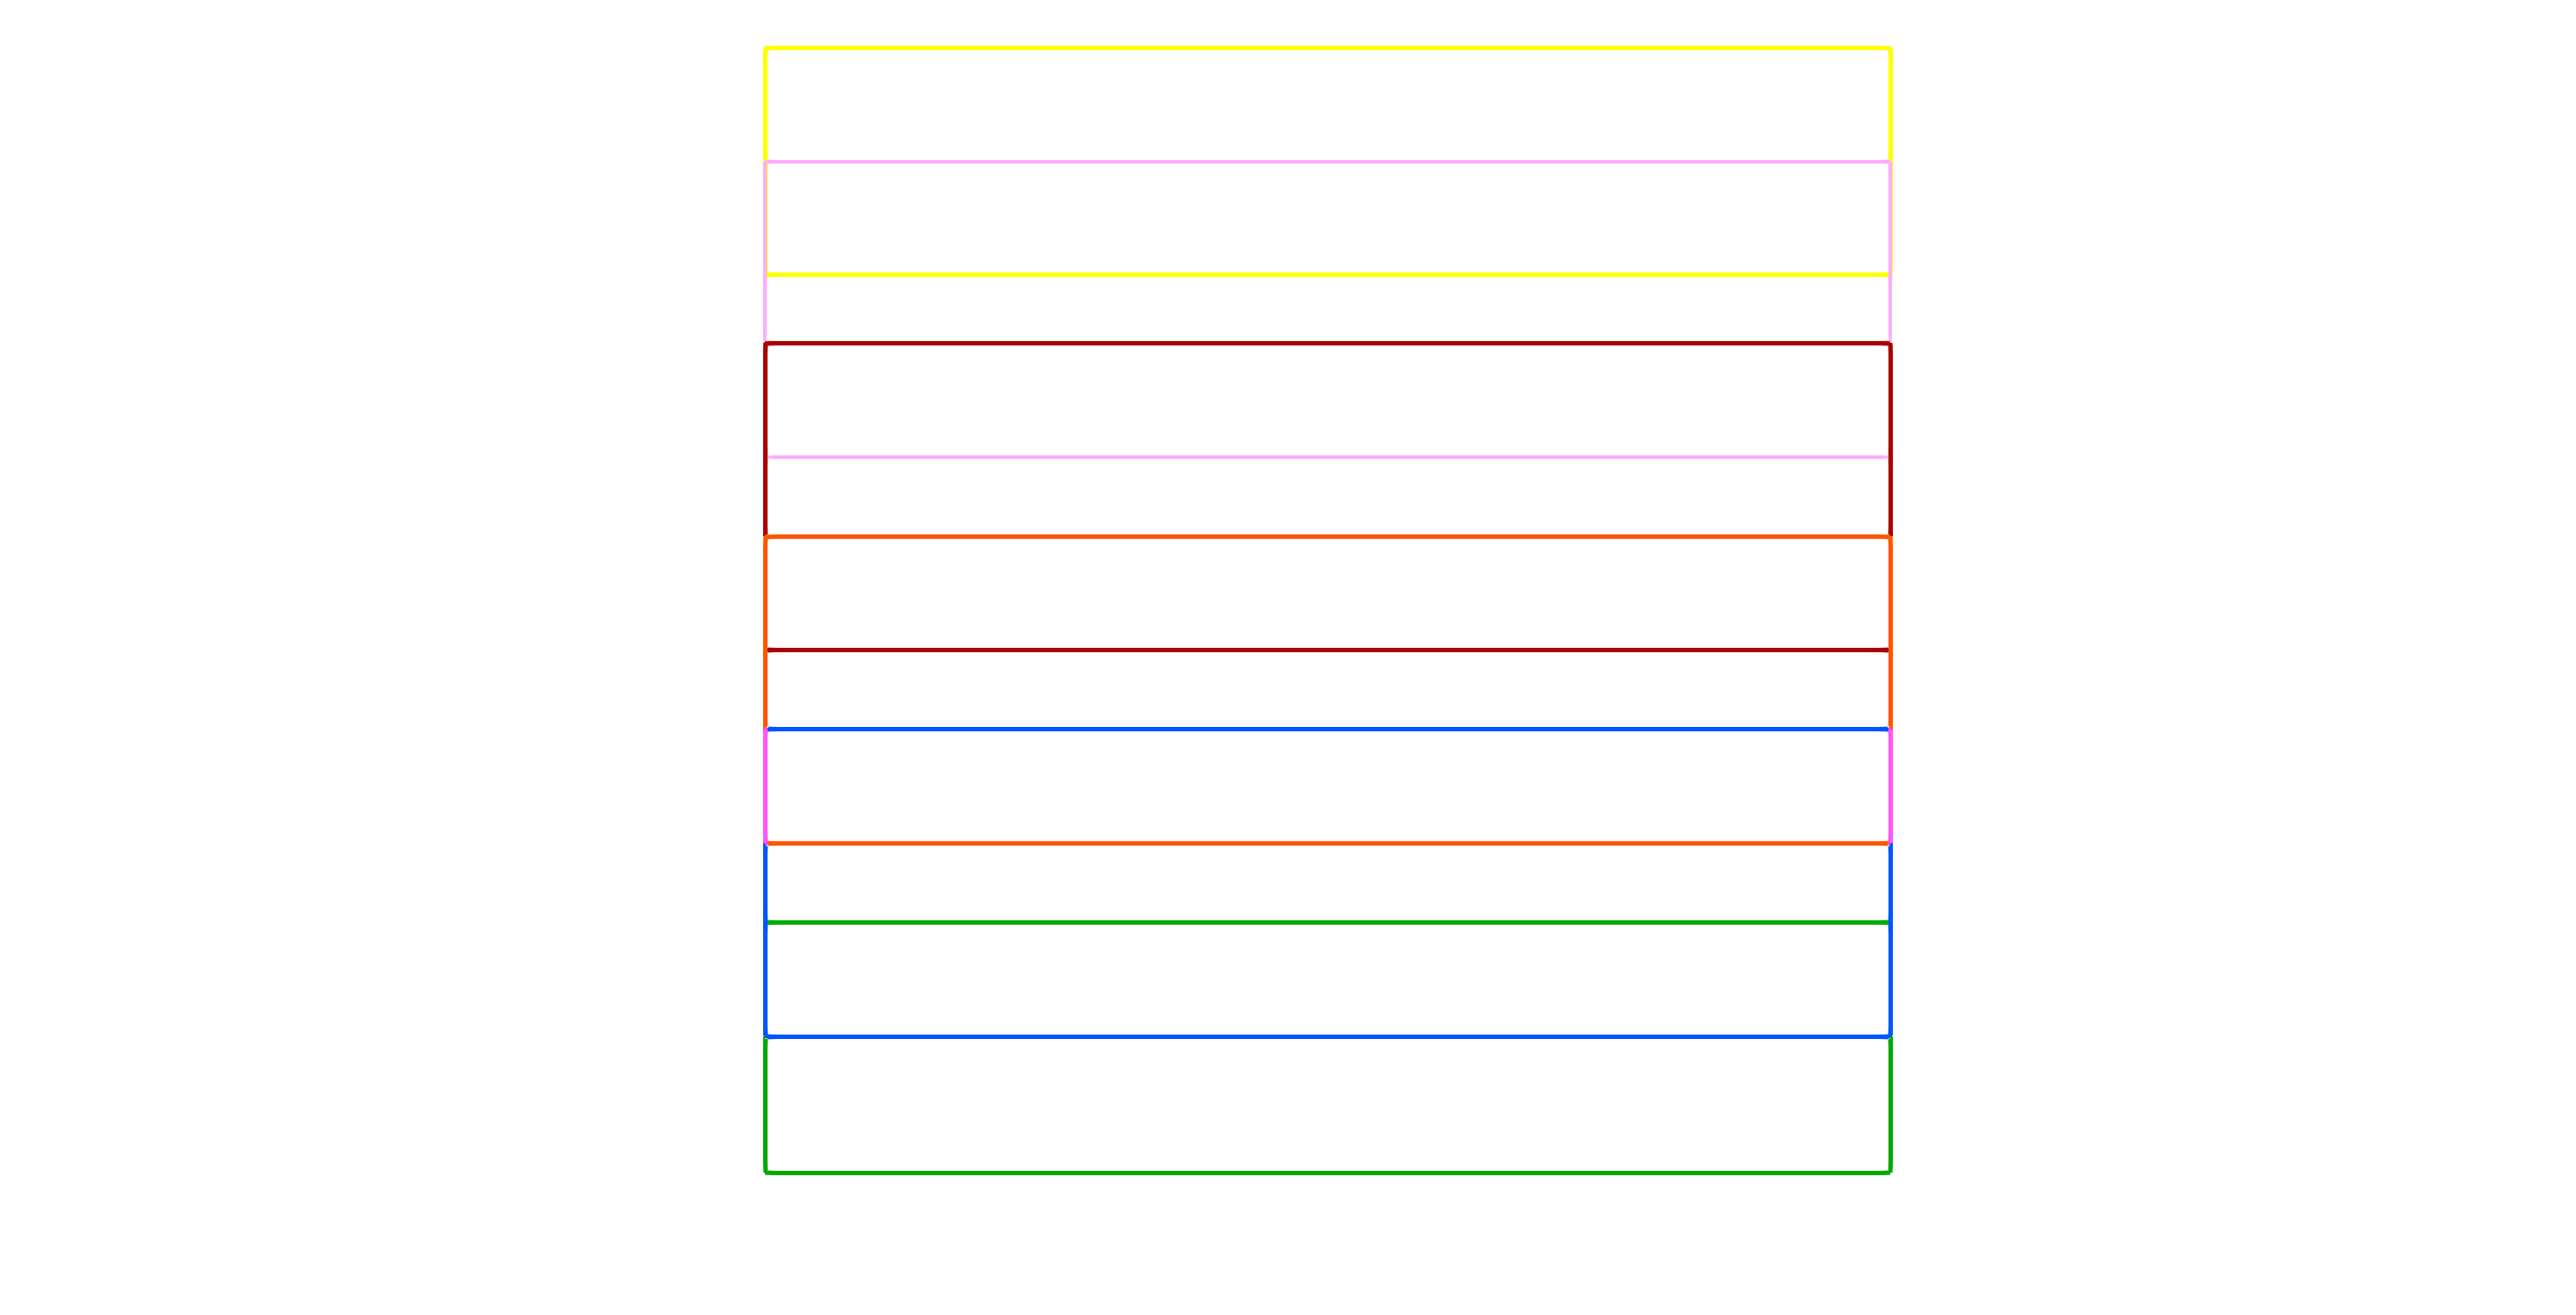
\includegraphics[width=1.5\textwidth]{row_6.png}
		\caption{Row}
	\end{subfigure}
\end{figure}
\begin{figure}[H]\ContinuedFloat
	\begin{subfigure}[b]{0.45\textwidth}
		\hspace{-2.5cm}
		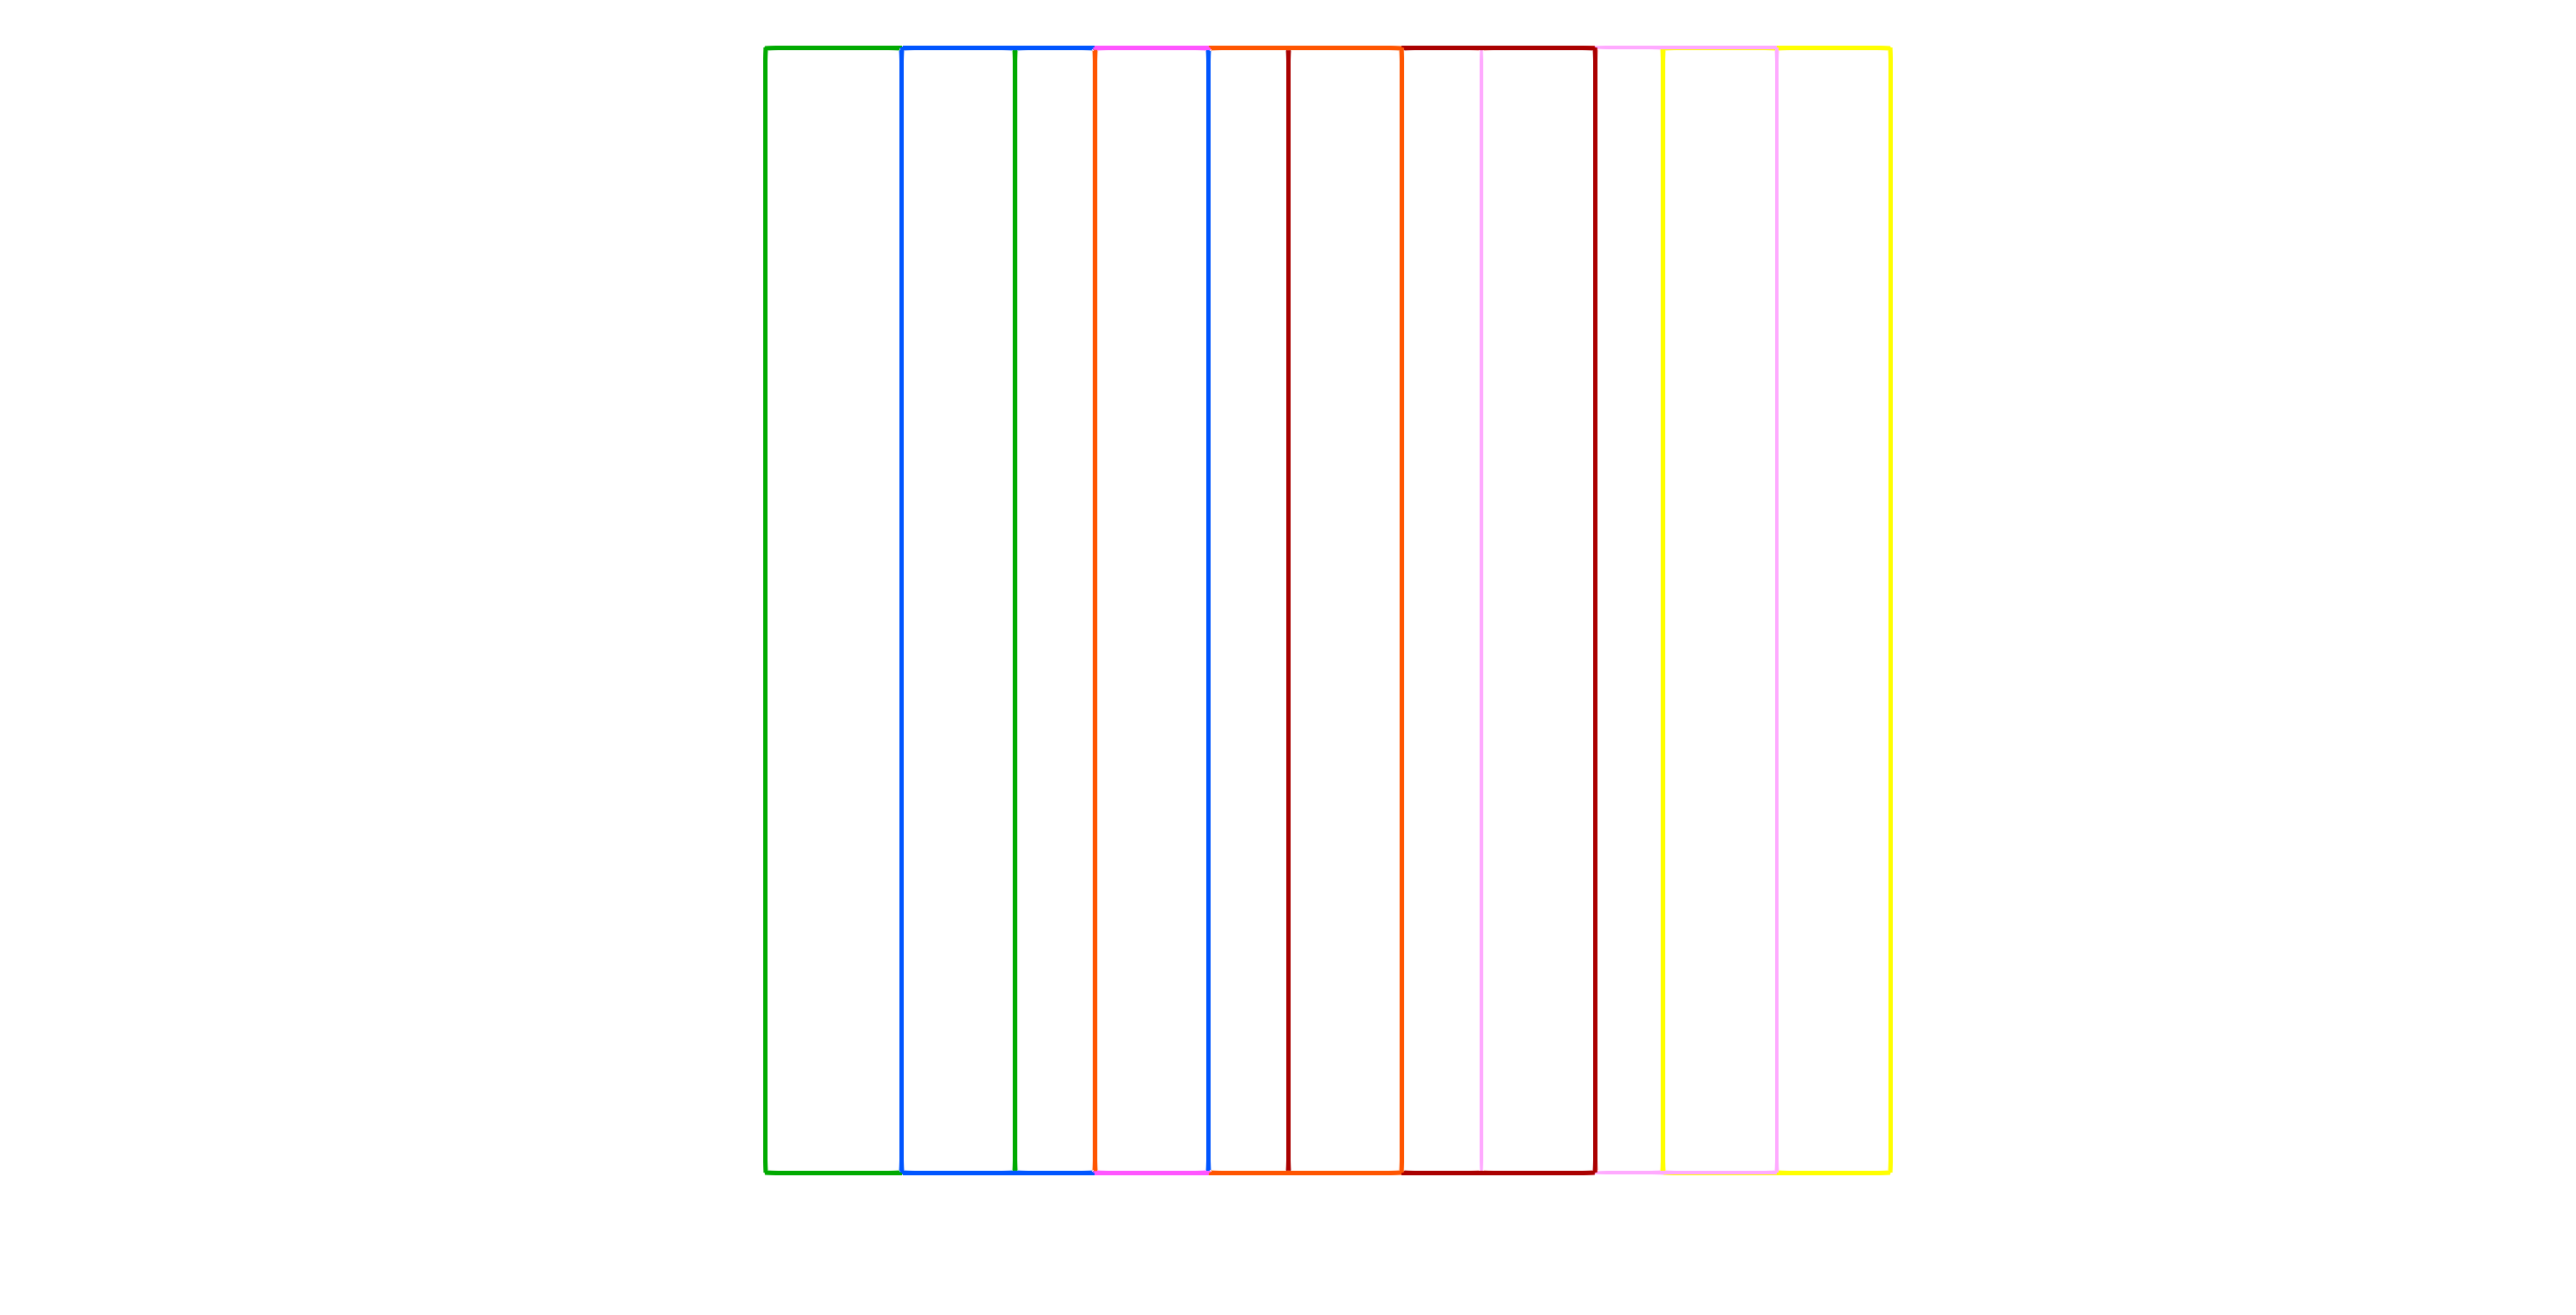
\includegraphics[width=1.5\textwidth]{column_6.png}
		\caption{Column}
	\end{subfigure}
\hfill
	\begin{subfigure}[b]{0.45\textwidth}
		\hspace{-2.5cm}
		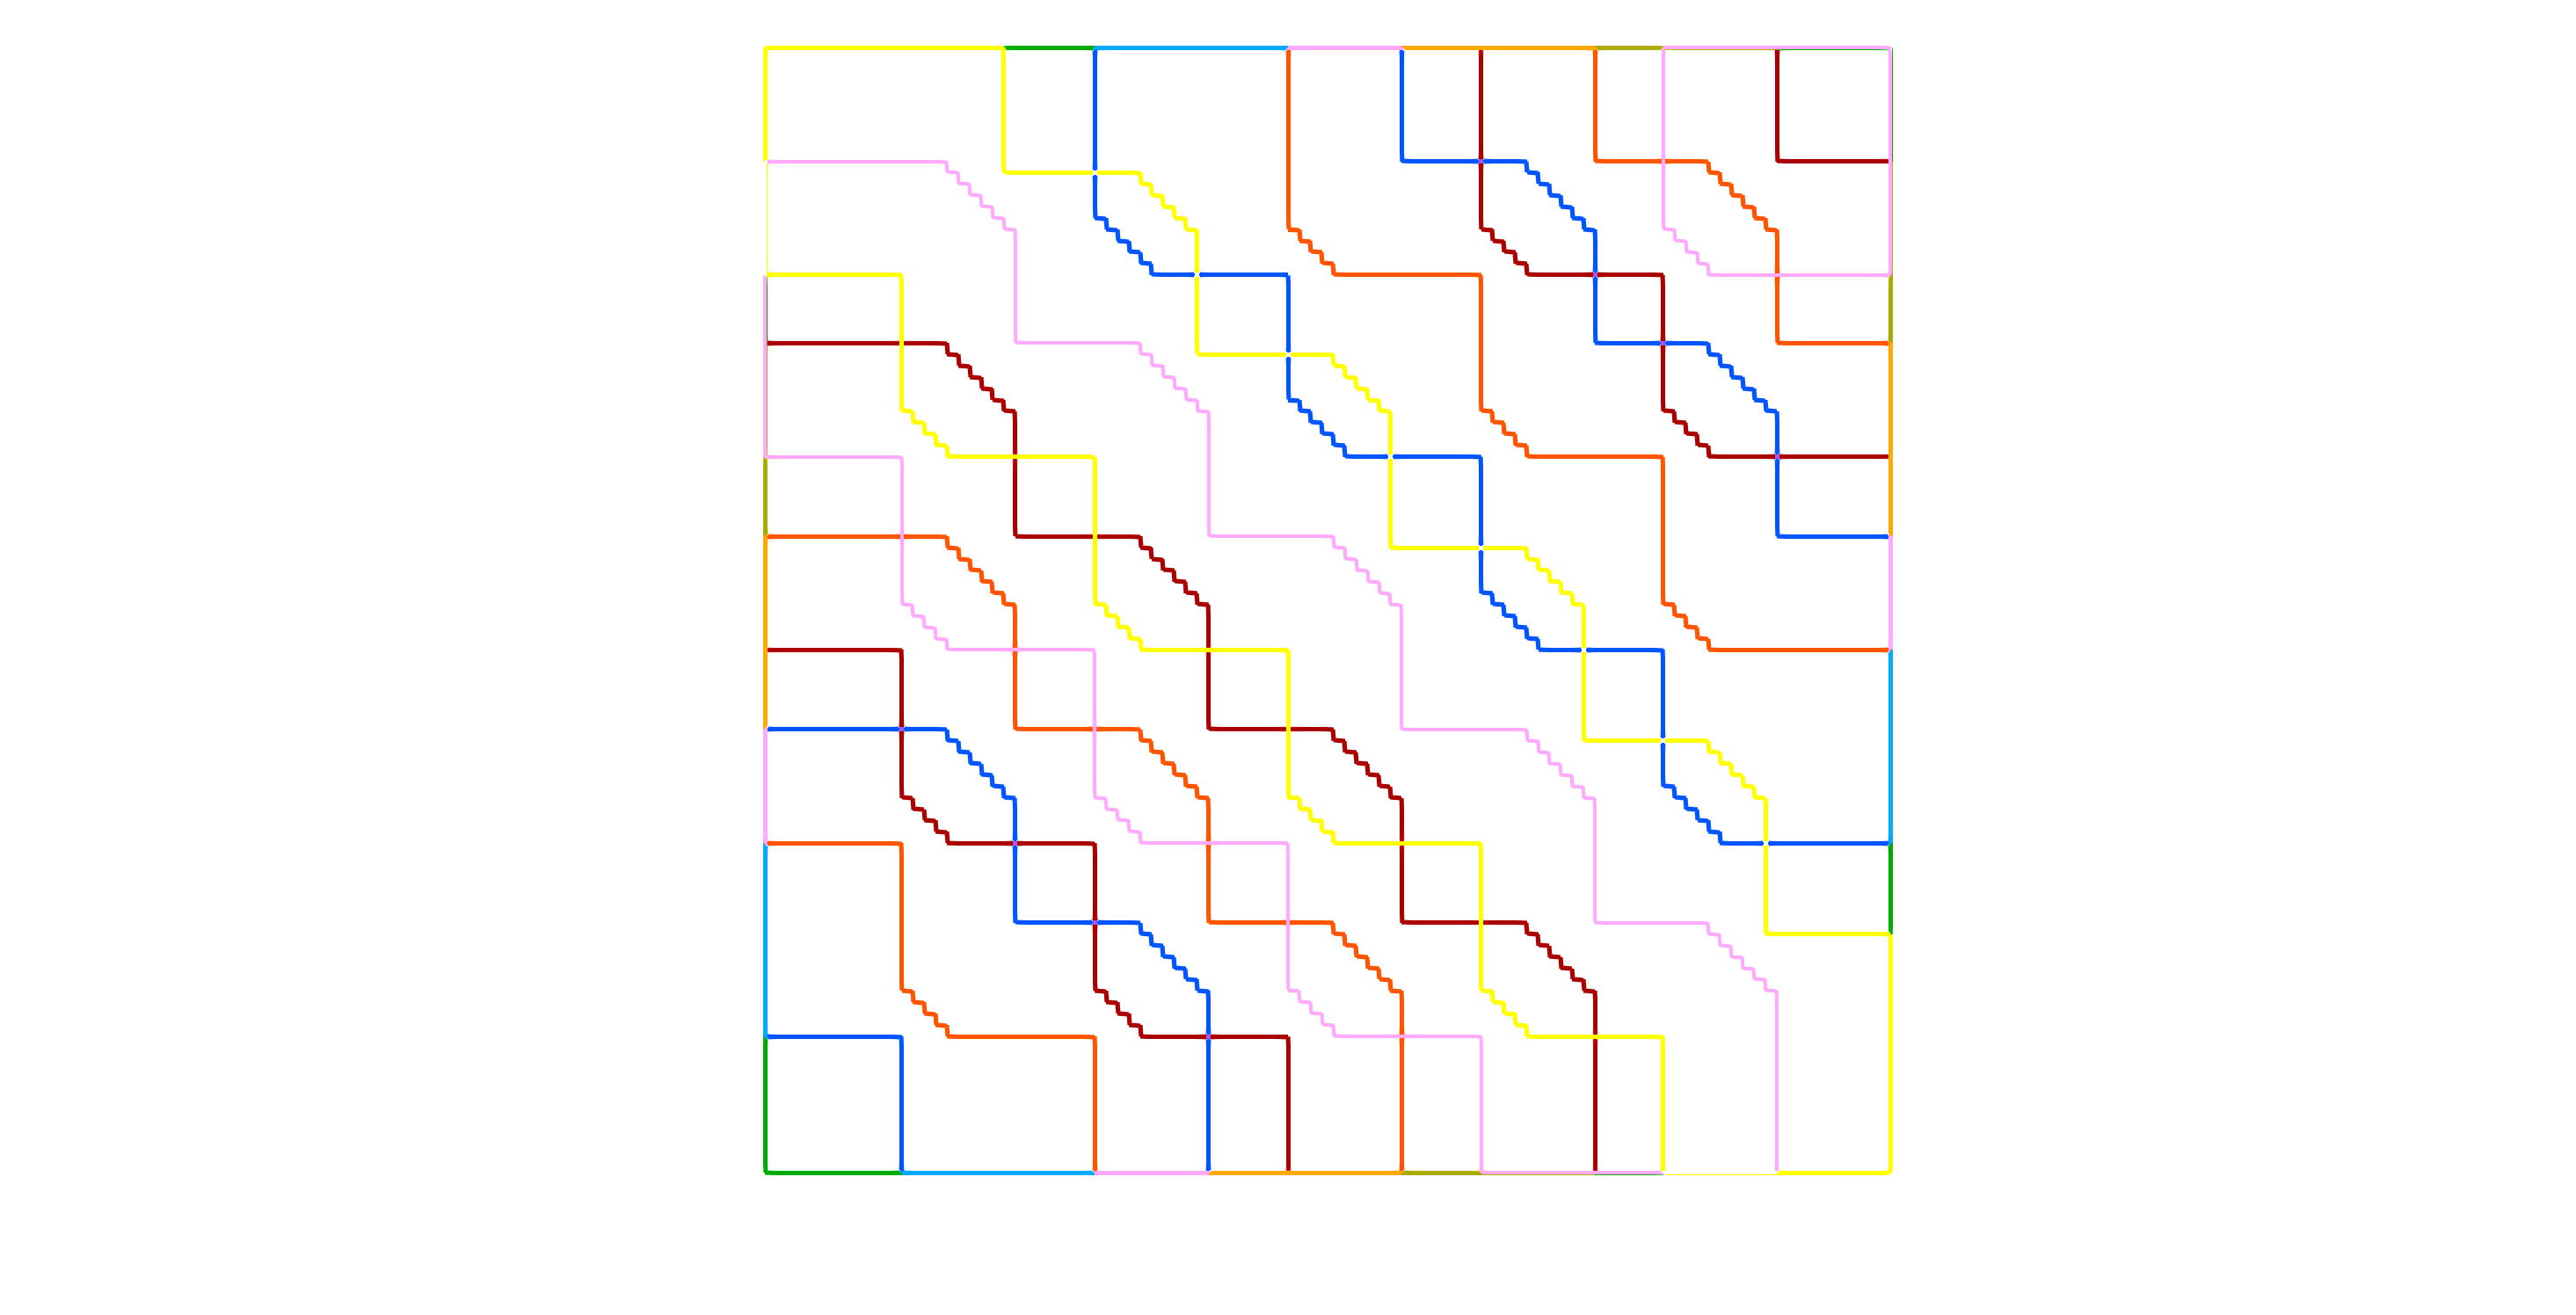
\includegraphics[width=1.5\textwidth]{board_6.png}
		\caption{Board}
	\end{subfigure}
	\caption{Les différents types de partitionnement, exemple 6 partitions, taille du recouvrement 5}
	\label{fig:typepartition}
\end{figure}
\noindent En pratique le recouvrement est établi après partitionnement en trois étapes :
\begin{enumerate}
	\item Nous partitionnons le graphe constitué des $n_x \times n_y$ points ($n_x$ et $n_y$ étant le nombre de points dans chaque direction sur le maillage initial).  À ce stade chaque point appartient à une et une seule partition.
	\item Un premier passage de la fonction d'agrandissement permet d'agrandir les partitions en les étendant sur les partitions voisines dont le numéro est plus grand. À l'issu de ceci toutes les partitions partagent leurs bords virtuels avec d'autres partitions.
	\item Ensuite nous itérons la fonction d'agrandissement autant de fois que la taille de recouvrement souhaité : pour chaque point de chaque partition nous colorions les voisins de la couleur du processeur courant.
\end{enumerate}
À l'issu de ces trois étapes nous obtenons des partitions de notre domaine $\Omega$ avec le recouvrement voulu. Par exemple, la figure \ref{fig:typepartition} explicite les différents algorithmes de partitionnement pour une même taille de recouvrement. Nous pouvons pointer dès maintenant l'importance du partitionnement : autant du point de vue des communications que du nombres d'itérations nécessaires pour résoudre notre problème initiale \eqref{eq:poisson} sous le critère dégagé précédemment.\\
\paragraph{Voronoï} La méthode de partitionnement par équilibrage du diagramme de Voronoï est sans doute la moins claire des méthodes présentées. Nous avons implémenté l'équilibrage par déplacement des générateurs ($N_p$ générateurs pour $N_p$ partitions) vers la moyenne de tous les points de la partition. Ensuite nous déduisons à quelle zone appartient le point par la recherche du générateur le plus proche. S'il y a un problème à souligner c'est bien celui-ci, cette recherche est faite à l'aide de la norme $\ell^2$ et non en terme de distance d'arêtes. Si nous voulions améliorer cette méthode il faudrait changer ceci. Il est important de noter pour la suite que Metis utilise un algorithme de \textit{k-mean} qui est basé sur l'algorithme de Lloyd, le c\oe ur même de notre équilibrage.

\subsubsection{Sans superposition de recouvrements}
\noindent Nous nous intéressons maintenant à la mise en \oe uvre pratique d'un recouvrement et d'échanges de conditions aux bords virtuels. Dans le code nous avons choisi de faire des recouvrements de taille impaires dans chaque direction (ceci est une condition directe de l'algorithme de recouvrement présenté à la sous-section précédente). Nous illustrons l'échange de valeurs en une dimension par le schéma suivant
\begin{figure}[H]
	\incfig{0.6}{appart}
	\caption{Communication de conditions aux bords virtuels.}
\end{figure}
\noindent Ce schéma comporte des cercles : ce sont des points qui ne demandent pas de traitement particulier, leur(s) couleur(s) désigne le processeur auquel ils appartiennent. Par exemple, le point colorié en \textcolor{red}{rouge} et \textcolor[RGB]{0, 140, 0}{vert}  est \textbf{partagé} par les deux processeurs \textcolor{red}{rouge} et \textcolor[RGB]{0, 140, 0}{vert}. Le schéma comporte aussi deux carrés : ce sont des points d'échanges. Les couleurs désigne aussi les processeurs auxquels appartient le point. La couleur intérieure désigne la couleur du processeur qui \textit{envoie} la condition au bord et la couleur extérieure désigne la couleur du processeur qui \textit{reçoit} la condition au bord. Nous faisons un récapitulatif sur le graphe suivant, c'est la version simplifiée de ce qui se passe dans le code mais l'idée reste la même.
\begin{figure}[H]
	\centering
	\begin{tikzpicture}
	[
	grow                    = right,
	sibling distance        = 6em,
	level distance          = 10em,
	edge from parent/.style = {draw, -latex},
	every node/.style       = {font=\footnotesize},
	sloped
	]
	\node [root] {Forme}
	child { node [env] {Ma couleur ?}
		child { node [dummy] {}
			edge from parent node [above, align=center] {Couleur}
			node [below] {intérieure} }
		edge from parent node [below] {Cercle} }
	child { node [env] {Ma couleur ?}
		child { node [env] {Receveur}
			edge from parent node [above, align=center] {Couleur}
			node [below] {extérieure} }
		child { node [env] {Envoyeur}
			edge from parent node [above, align=center]
			{Couleur}
			node [below] {intérieure}}
		edge from parent node [above] {Carré} };
	\end{tikzpicture}
	\caption{Arbre de catégorisation sans superposition de recouvrement.}
\end{figure}

\subsubsection{Avec superposition de recouvrements}
\noindent Un cas pathologique est apparu au cours de nos tests numériques et de nos différentes techniques de partitionnement. Que faire quand au moins deux processeurs tombent dans la case "envoyeur" de l'arbre de décision précédent pour un même point ?  L'exemple est illustré sur la figure ci-après
\begin{figure}[H]
	\incfig{0.6}{youngest}
	\caption{La règle du plus jeune envoyeur.}
\end{figure}
\noindent La règle la plus simple à mettre en \oe uvre nécéssite un ordre entre les différentes partitions et donc entre les différents numéros de processeurs pour être valide. La règle, intuitive, qui en découle, que nous nommerons la règle du plus jeune envoyeur est la suivante 
\begin{equation}
	\text{\textit{Je suis un \textbf{envoyeur} si aucun des processeurs avant moi n'est un \textbf{envoyeur}}}.\label{eq:younguest}
\end{equation}
L'arbre de décision est modifié en conséquence
\begin{figure}[H]
	\centering
	\begin{tikzpicture}
	[
	grow                    = right,
	sibling distance        = 6em,
	level distance          = 10em,
	edge from parent/.style = {draw, -latex},
	every node/.style       = {font=\footnotesize},
	sloped
	]
	\node [root] {Forme}
	child { node [env] {Ma couleur ?}
		child { node [dummy] {}
			edge from parent node [above, align=center] {Couleur}
			node [below] {intérieure} }
		edge from parent node [below] {Cercle} }
	child { node [env] {Ma couleur ?}
		child { node [env] {Receveur}
			edge from parent node [above, align=center] {Couleur}
			node [below] {extérieure} }
		child { node [env] {Je suis le plus jeune ?}
			child { node [dummy] {}
				edge from parent node [below] {Non} }
			child { node [env] {Envoyeur}
				edge from parent node [below] {Oui} }
			edge from parent node [above, align=center]
			{Couleur}
			node [below] {intérieure}}
		edge from parent node [above] {Carré} };
	\end{tikzpicture}
	\caption{Arbre de catégorisation version "plus jeune envoyeur".}
\end{figure}
\noindent Cette technique, bien que simpliste, permet de définir un \textbf{unique processeur envoyeur} et une liste de \textbf{processeurs receveurs} par point. Nous rappelons ici qu'une condition de type Robin dans un coin de la partition est automatiquement transformé en condition de Dirichlet (voir la section précédente).\\

\subsubsection{Le format ".lyra"} 
\noindent Nous présentons ici le format de maillage (aisément modifiable) dont nous avons précédemment parlé et qui est la passerelle entre les différents exécutables de la bibliothèque \textbf{Lyra}.

\begin{table}[H]
	\centering
	\fbox{\parbox{\dimexpr\linewidth-2\fboxsep-2\fboxrule\relax}{
			\ttfamily
			number-of-points\\
			coor-x coor-y coor-z global-num tag tag-infos $\backslash\backslash$ for each point\\
			...\\
			number-of-cells\\
			vertex-1 vertex-2 vertex-3 vertex-4 $\backslash\backslash$ for each cell\\
			...
	}}%
	\caption{Le format ".lyra"}
\end{table}
\noindent où
\begin{itemize}
	\item \texttt{coor-x coor-y coor-z} sont les coordonnées du point
	\item \texttt{global-num} est le numéro global du point sur le maillage initial (avant partitionnement), ce numéro est essentiel car il servira dans l'ordre des réceptions/envois avec MPI \footnote{MPI : \url{https://www.mpich.org/}}
	\item \texttt{tag} est un nombre au format binaire représentant tous les tags du point. Voici les tags possibles
	\begin{table}[H]
		\centering
		\begin{tabular}{|l|c|c|c|}
			\hline
			\multicolumn{1}{|c|}{\cellcolor[HTML]{FFFFFF}{\color[HTML]{CB0000} \texttt{Tag}}} & Valeur & Digit & Sur cette partition, je suis     \\ \hline
			\rowcolor[HTML]{C0C0C0} 
			{\color[HTML]{CB0000} \texttt{PT\_NONE}}                                          & 0x0    & 1     & un simple point                  \\ \hline
			\cellcolor[HTML]{FFFFFF}{\color[HTML]{CB0000} \texttt{PT\_SHARED}}                & 0x1    & 1     & partagé avec une autre partition \\ \hline
			\rowcolor[HTML]{C0C0C0} 
			{\color[HTML]{CB0000} \texttt{PT\_PHYSICAL}}                                      & 0x2    & 2     & un point de bord physique        \\ \hline
			\cellcolor[HTML]{FFFFFF}{\color[HTML]{CB0000} \texttt{PT\_VIRTUAL}}               & 0x4    & 3     & un point de bord virtuel         \\ \hline
			\rowcolor[HTML]{C0C0C0} 
			{\color[HTML]{CB0000} \texttt{PT\_SEND}}                                          & 0x8    & 4     & un point envoyeur                \\ \hline
			\cellcolor[HTML]{FFFFFF}{\color[HTML]{CB0000} \texttt{PT\_RECEIVE}}               & 0x10   & 5     & un point receveur                \\ \hline
			\rowcolor[HTML]{C0C0C0} 
			{\color[HTML]{CB0000} \texttt{PT\_DIRICHLET}} &
			0x20 &
			6 &
			\begin{tabular}[c]{@{}c@{}}un point où il faut imposer \\ une condition de type Dirichlet\end{tabular} \\ \hline
			\cellcolor[HTML]{FFFFFF}{\color[HTML]{CB0000} \texttt{PT\_NEUMANN}} &
			0x40 &
			7 &
			\begin{tabular}[c]{@{}c@{}}un point où il faut imposer \\ une condition de type Neumann\end{tabular} \\ \hline
			\rowcolor[HTML]{FFCC67} 
			{\color[HTML]{CB0000} \texttt{\begin{tabular}[c]{@{}l@{}}PT\_ROBIN = \\ PT\_DIRICHLET | PT\_NEUMANN\end{tabular}}} &
			0x60 &
			6 \& 7 &
			\begin{tabular}[c]{@{}c@{}}un point où il faut imposer \\ une condition de type Robin\end{tabular} \\ \hline
		\end{tabular}
		\caption{L'énumération \texttt{PTAG}}
	\end{table}
	Par exemple, le tag \texttt{1101101} signifie  \texttt{PT\_ROBIN} |  \texttt{PT\_SEND} |  \texttt{PT\_VIRTUAL} | \texttt{PT\_SHARED}.
	\item \texttt{tag-infos} sont les informations additionnelles nécessaires aux communications, elles sont donc uniquement déterminé par les tags \texttt{PT\_SEND} et \texttt{PT\_RECEIVE} :
	\begin{itemize}
		\item Si \texttt{PT\_SEND} alors il faut \texttt{number-of-receivers [id-proc dir-normal-outward]...}\\
			où \texttt{dir-normal-outward} vaut
			\begin{center}
				\texttt{\{LEFT = 0, RIGHT = 1, UP = 2, BOTTOM = 4, NOT\_SET = 5\}}
			\end{center}
			 et sera utilisé pour la condition de type Robin.
		\item Si \texttt{PT\_RECEIVE} alors il faut uniquement \texttt{id-proc-sender}
	\end{itemize}
\end{itemize}

\subsection{Résultats}
\noindent Nous présentons dans cette section divers résultats obtenus. Dans un premier temps rappelons les deux définitions utilisées en calcul parallèle pour déterminer la \textit{performance} d'un code parallélisé par rapport au code séquentiel. Nous introduisons les notations $\text{time}_{1}$ désignant le temps série et $\text{time}_{N_p}$ le temps parallèle en utilisant $N_p$ processus.
\begin{align*}
	\text{Speed-up}\left(N_p\right) &= \frac{\text{charge totale}}{\underset{\text{procs}\in N_p}{\max} ~\text{charge}} \approx \frac{\text{time}_{1}}{\text{time}_{N_p}} \leq N_p\\
	\text{Efficacité}\left(N_p\right) &= \frac{\text{Speed-up}\left(N_p\right)}{N_p} \approx \frac{\text{time}_{1}}{N_p \times \text{time}_{N_p}} \leq 1
\end{align*}
où $N_p$ est le nombre de processeurs utilisés. Nous ferons toujours la distinction entre la définition théorique et le résultat obtenu en pratique.\\
Nous introduisons aussi ce que nous appellerons le speed-up et l'efficacité normalisés à $\alpha$ processus comme :
\begin{align*}
\text{Speed-up-}\alpha\left(N_p\right) &= \frac{\alpha\times \text{Speed-up} \left(\alpha\right)}{\text{Speed-up} \left(N_p\right)} \approx \frac{\alpha \times \text{time}_{\alpha}}{\text{time}_{N_p}} \leq N_p\\
\text{Efficacité-}\alpha\left(N_p\right) &= \frac{\text{Speed-up-}\alpha\left(N_p\right)}{N_p} \approx \frac{\alpha \times \text{time}_\alpha}{N_p \times \text{time}_{N_p}} \leq 1
\end{align*}
Par ailleurs, les différentes simulations ont été effectuées sur PlaFRIM avec différents scripts. Le solveur Lyra a été configuré comme suit
\begin{itemize}
	\item le gradient conjugué et le bigradient conjugué stabilisé à une tolérance de $10^{-10}$,
	\item les itérations de Schwarz s'arrêtent lorsque le maximum de la différence entre deux solutions numériques est de $10^{-3}$. Cette valeur est réduite et sommée sur chaque partition.
\end{itemize}
\subsubsection{L'effet du partitionnement}
\noindent Avant de comparer plus en profondeur le speed-up et l'efficacité de notre code, nous proposons de regarder succinctement l'effet des différents choix que nous avons fait lors du partitionnement.\\

\noindent \textit{La règle du plus jeune envoyeur} \eqref{eq:younguest} n'est pas étudié ici même si nous sommes conscient que cette \textbf{règle} est purement empirique et qu'il se peut qu'un choix plus stratégique se dégage au cours d'explorations : cela dépendrait certainement de la taille du recouvrement et du problème étudié.\\

\noindent La conversion de Robin à Dirichlet concernant les coins a un impact non négligeable au vu de nos simulations (l'effet Dirichlet-Robin est expliqué dans la suite). Regardons donc le taux de conversion selon la méthode de partitionnement choisi. Pour cet exemple nous avons utilisé un maillage de $200\times 200$ que nous avons partitionné avec plusieurs méthodes avec une taille de recouvrement de 5 mailles (à multiplier par deux selon l'algorithme établi précédemment). Il est important de préciser qu'à partir de $20$ partitions nombre de méthodes produisent des domaines entièrement partagés : par exemple une division en $20$ lignes produit des partitions avant recouvrement de taille $10$ et il est inévitable que le recouvrement à droite rejoigne celui de gauche avec notre taille prescrite.
\begin{figure}[H]
	\centering
	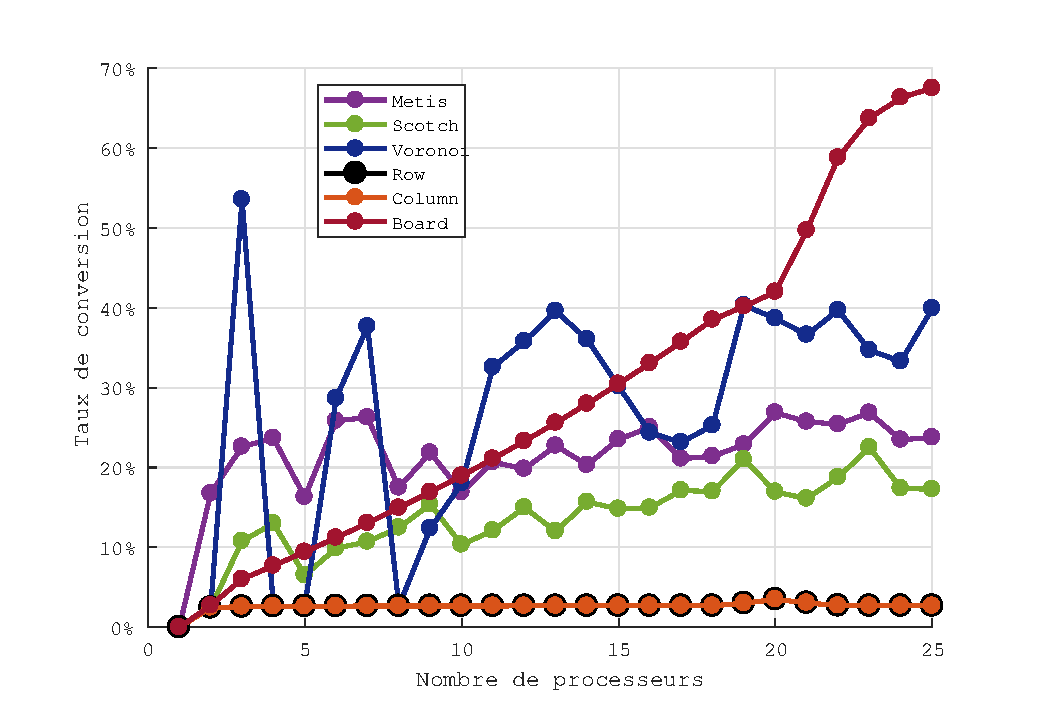
\includegraphics[width=0.8\textwidth]{taudeconversion.eps}
	\caption{Taux de conversion de Robin vers Dirichlet.}
\end{figure}
Plusieurs observations sont à faire ici : 
\begin{itemize}
	\item le partitionnement en lignes ou colonnes semble être la méthode qui transforme le moins de Robin en Dirichlet et cela même quand le nombre de partitions augmente : ceci s'explique car ces méthodes suivent la discrétisation (topographie) du maillage, nous dirons ici que \textit{le partitionnement est fidèle au maillage}.
	\item Scotch semble donner des partitions plus fidèle que Metis même si pour ces deux méthodes nous restons en dessous de la barre des $30\%$ ce qui est compréhensible car autant l'un que l'autre ont une \textbf{véritable} implémentation de partitionnement de graphe avec des méthodes qui ont fait leurs preuves.
	\item le partitionnement selon un l'uniformisation diagramme de Voronoï semble être la plus aléatoire et cela s'explique tout naturellement par rapport au \textit{nombre de partitions demandées}. Nous pourrions aller chercher du côté des carrés parfaits pour trouver une explication plus théorique.
	\item Le partitionnement en damier semble être linéaire jusqu'à atteindre le nombre de partitions fatidique exposé précédemment. Au cours de nos tests nous avons remarqué que cette droite semble être de moins en moins pentue à mesure que le nombre de points de discrétisation augmente, cette méthode semble être un bon compromis à celle de Voronoï par exemple.
\end{itemize}
\noindent Regardons maintenant toutes ces méthodes d'un point de vue plus informatique : la taille des messages à faire transiter (le nombre de communications nécessaires). En effet le temps de communication (a fortiori la taille des messages) est une donnée importante à prendre en compte. Cet taille correspond en pratique au nombre de points définissant les interfaces entre les partitions.
\begin{figure}[H]
	\centering
	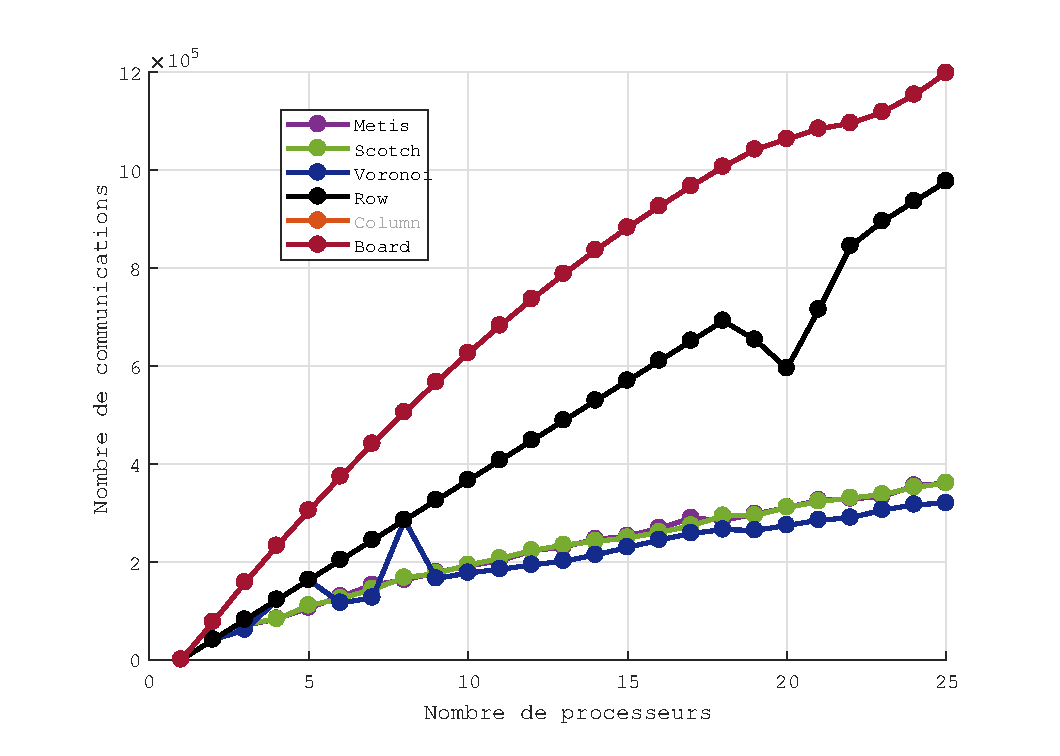
\includegraphics[width=0.8\textwidth]{communic.eps}
	\caption{Nombre de communications nécessaires à une itération de Schwarz maillage $200\times200$.}
\end{figure}
\noindent La méthode de Voronoï est ici plus que surprenante : elle demande pratiquement autant de communication qu'un partitionnement fidèle au maillage. Le partitionnement en damier est sans conteste la méthode qui demande le plus de communications, tandis que partitionner en ligne ou colonne semble moins favorable tout à coup. \\
Au vu des deux comparaisons il semble qu'il vaille mieux partitionner avec Metis ou Scotch. Il nous faut maintenant valider toutes ces remarques à l'aide des indicateurs de performances établis en début de section.
\vspace{-9mm}
\subsubsection{Résolution $300\times 300$, recouvrement de taille 5}
\vspace{-7mm}
\begin{figure}[H]
	\centering
	\begin{subfigure}[t]{0.45\textwidth}
	\centering
	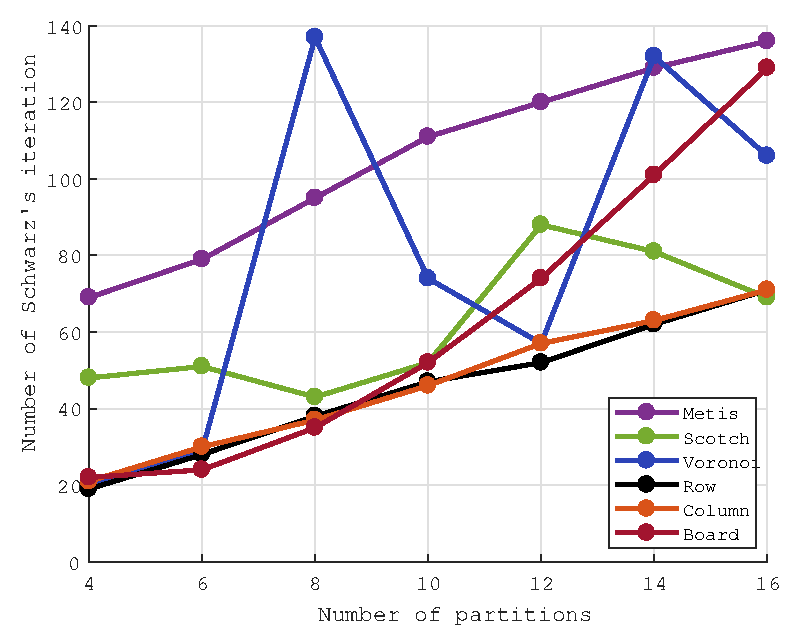
\includegraphics[width=\textwidth]{robin_300x300_5_iter.eps}
%	\caption{Robin}
	\end{subfigure}
	\hfill
	\begin{subfigure}[t]{0.45\textwidth}
	\centering
	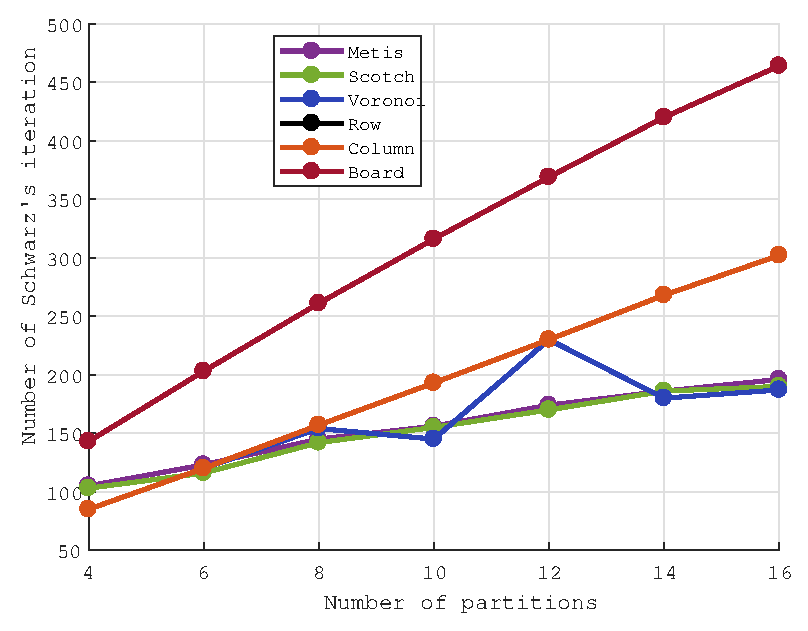
\includegraphics[width=\textwidth]{dirichlet_300x300_5_iter.eps}
%	\caption{Dirichlet}
	\end{subfigure}
\end{figure}
\vspace{-9mm}
\begin{figure}[H]\ContinuedFloat
	\begin{subfigure}[t]{0.45\textwidth}
		\centering
		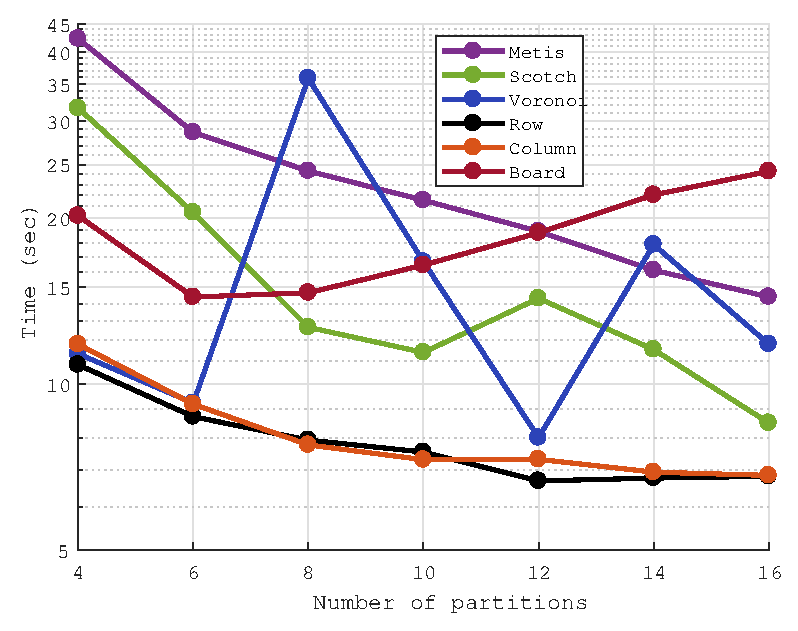
\includegraphics[width=\textwidth]{robin_300x300_5_time.eps}
%		\caption{Robin}
	\end{subfigure}
	\hfill
	\begin{subfigure}[t]{0.45\textwidth}
		\centering
		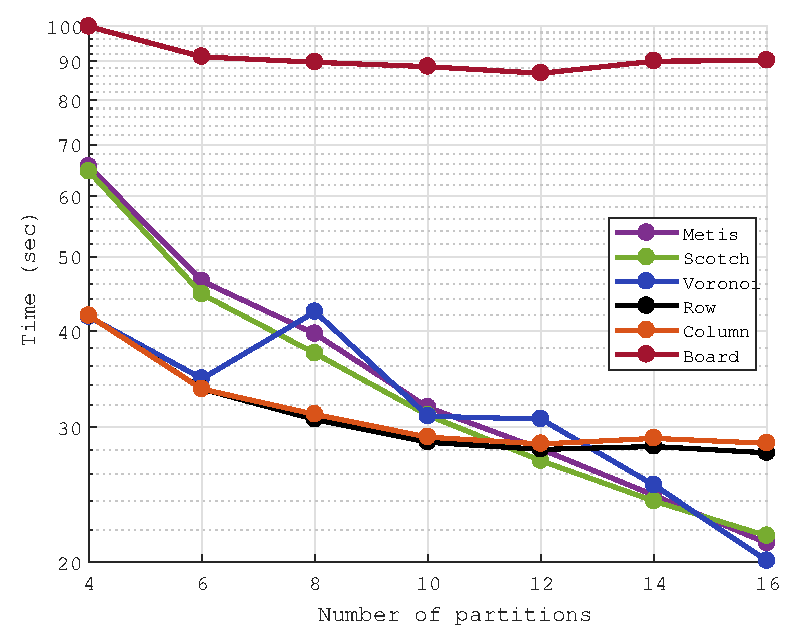
\includegraphics[width=\textwidth]{dirichlet_300x300_5_time.eps}
%		\caption{Dirichlet}
	\end{subfigure}
\end{figure}
\vspace{-9mm}
\begin{figure}[H]\ContinuedFloat
	\begin{subfigure}[t]{0.45\textwidth}
		\centering
		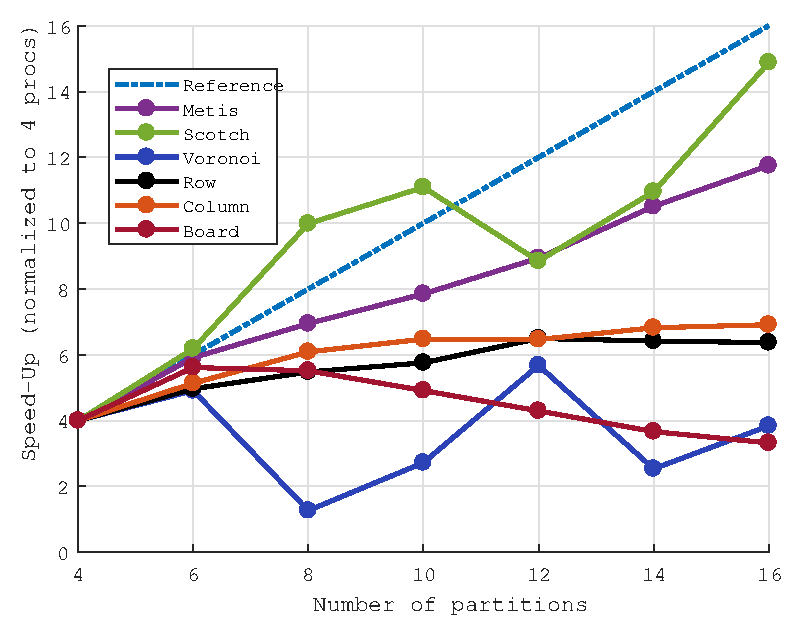
\includegraphics[width=\textwidth]{robin_300x300_5_speedup.eps}
%		\caption{Robin}
	\end{subfigure}
	\hfill
	\begin{subfigure}[t]{0.45\textwidth}
		\centering
		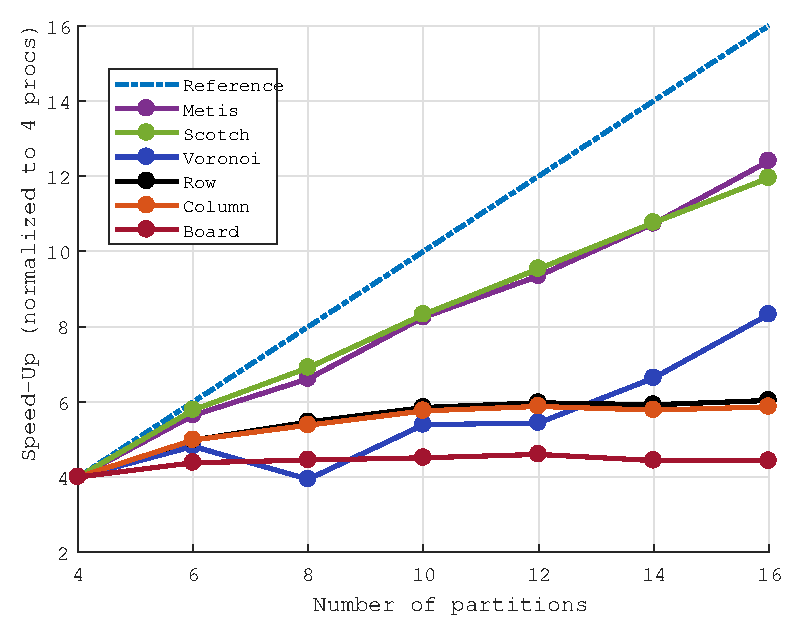
\includegraphics[width=\textwidth]{dirichlet_300x300_5_speedup.eps}
%		\caption{Dirichlet}
	\end{subfigure}
\end{figure}
\vspace*{-14mm}
\begin{figure}[H]\ContinuedFloat
	\begin{subfigure}[t]{0.45\textwidth}
		\centering
		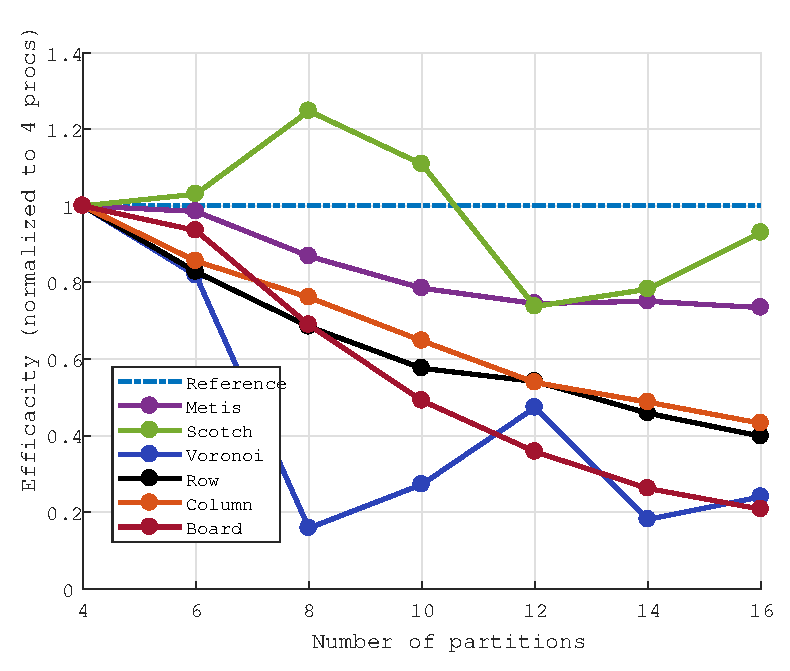
\includegraphics[width=\textwidth]{robin_300x300_5_efficacity.eps}
%		\caption{Robin}
	\end{subfigure}
	\hfill
	\begin{subfigure}[t]{0.45\textwidth}
		\centering
		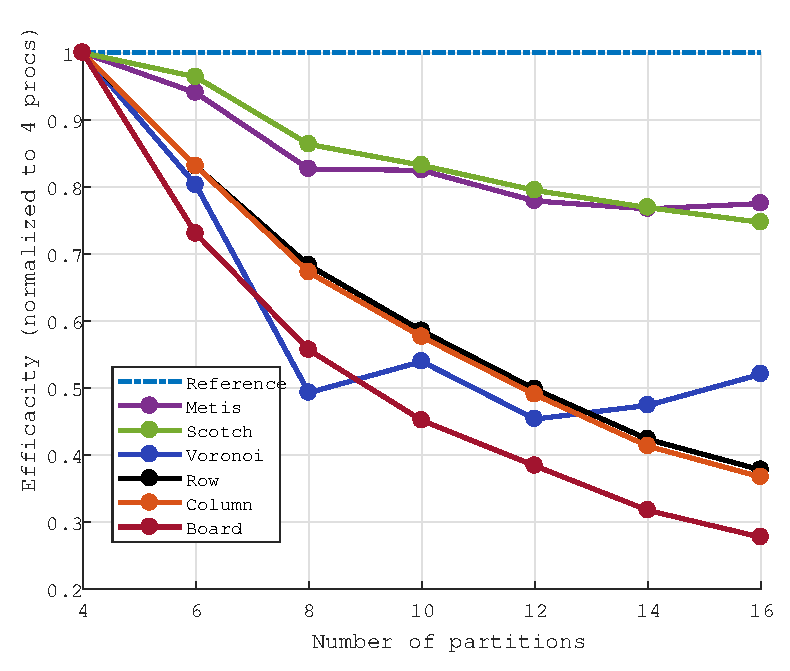
\includegraphics[width=\textwidth]{dirichlet_300x300_5_efficacity.eps}
%		\caption{Dirichlet}
	\end{subfigure}
	\caption{Analyse du $300\times300$ avec un recouvrement de taille 5. À droite Robin et à gauche Dirichlet.}
\end{figure}
\noindent Dans cet exemple de résolution nous avons utilisé tous les types de partitionnement disponibles. La méthode d'équilibrage type Voronoï semble celle qui donne les résultats les plus aléatoires pour des conditions de Robin, tandis que le partitionnement en damier est celui qui prend le plus de temps et le plus d'itérations avec des conditions de Dirichlet. La comparaison entre les conditions aux bords virtuels de Dirichlet et Robin est sans appel : utiliser les conditions de Robin divise par deux les temps de calcul globalement. Dans tous les cas, ce sont Metis et Scotch qui se distinguent le plus en terme d'efficacité ; Scotch allant jusqu'à une efficacité de 120\% pour des conditions de Robin !\\
Regardons maintenant ce que nos tests donnent lorsque nous augmentons le nombre de points sur le domaine (ie la charge pour chaque partition, presque deux fois plus).
\vspace*{-3mm}
\subsubsection{Résolution $400\times 400$, recouvrement de taille 5}
\vspace*{-3mm}
\begin{figure}[H]
	\centering
	\begin{subfigure}[t]{0.45\textwidth}
		\centering
		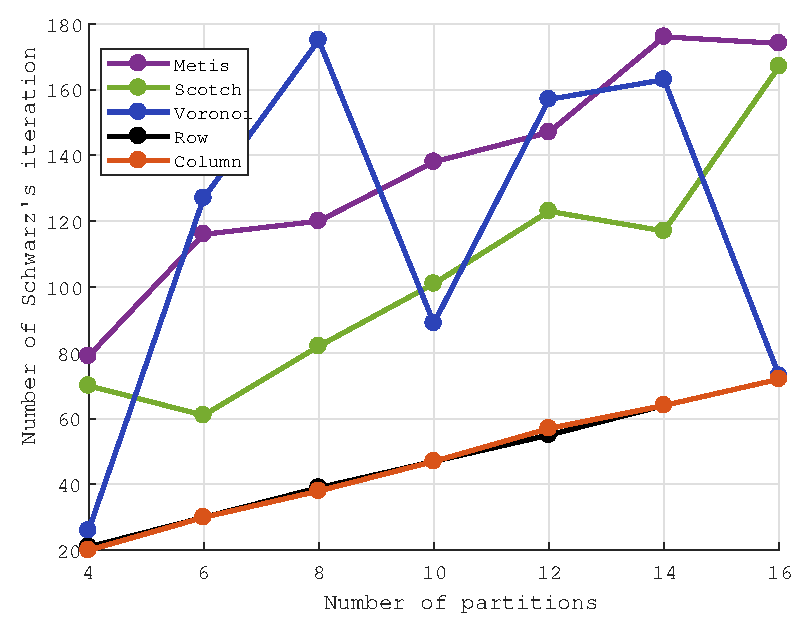
\includegraphics[width=\textwidth]{robin_400x400_5_iter.eps}
%		\caption{Robin}
	\end{subfigure}
	\hfill
	\begin{subfigure}[t]{0.45\textwidth}
		\centering
		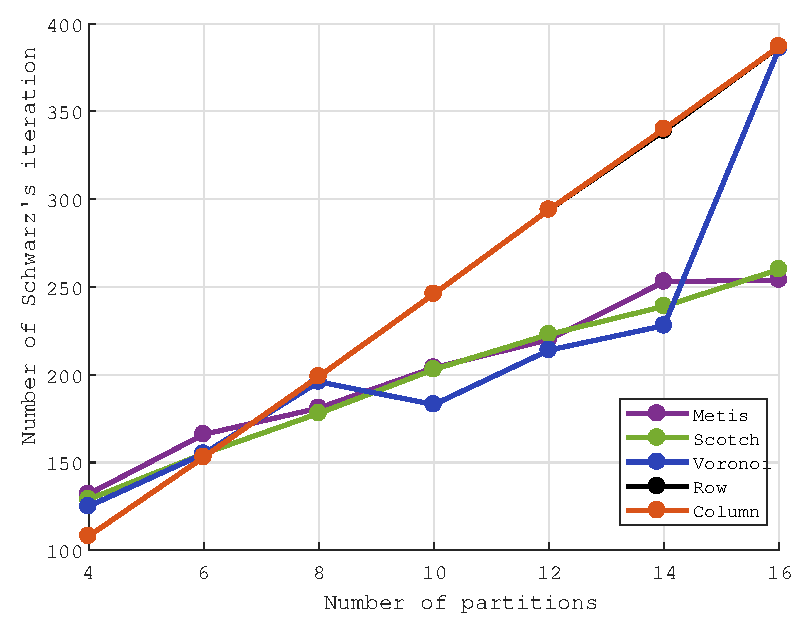
\includegraphics[width=\textwidth]{dirichlet_400x400_5_iter.eps}
%		\caption{Dirichlet}
	\end{subfigure}
\end{figure}
\vspace*{-8mm}
\begin{figure}[H]\ContinuedFloat
	\begin{subfigure}[t]{0.45\textwidth}
		\centering
		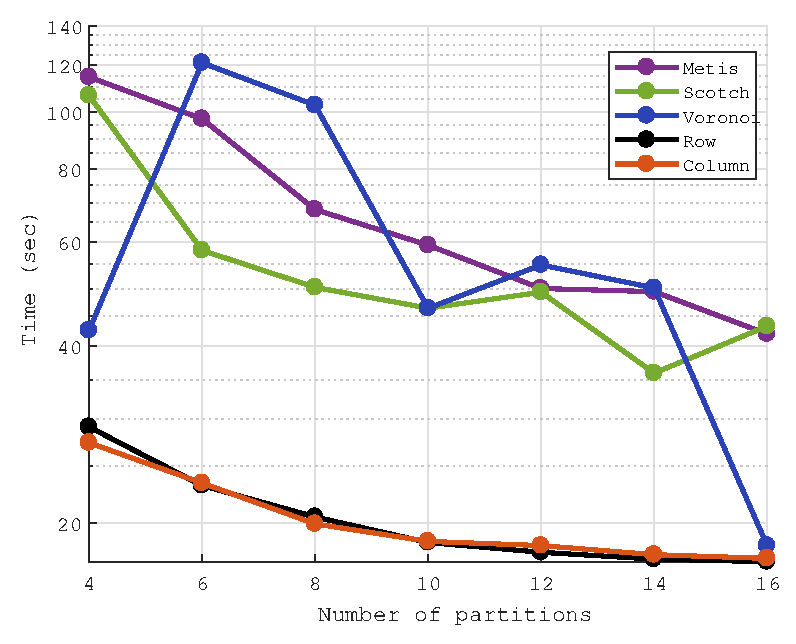
\includegraphics[width=\textwidth]{robin_400x400_5_time.eps}
%		\caption{Robin}
	\end{subfigure}
	\hfill
	\begin{subfigure}[t]{0.45\textwidth}
		\centering
		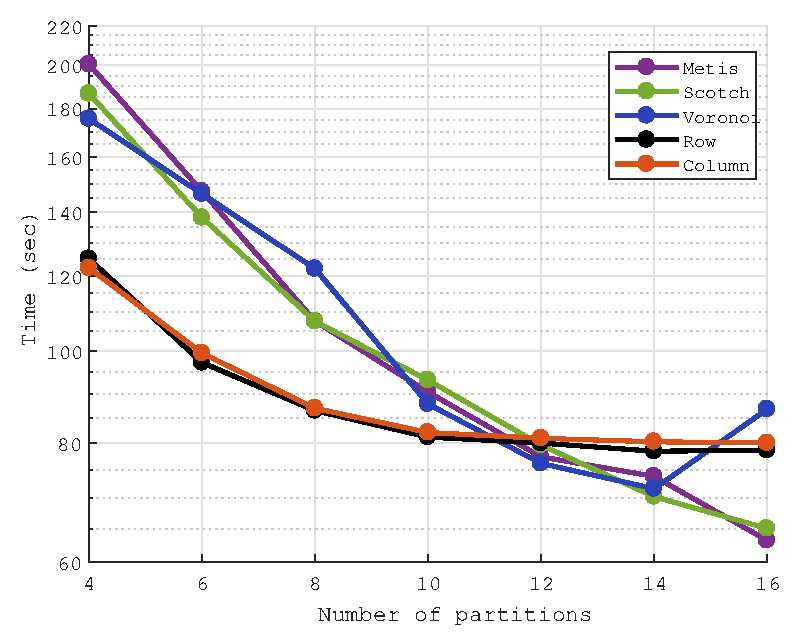
\includegraphics[width=\textwidth]{dirichlet_400x400_5_time.eps}
%		\caption{Dirichlet}
	\end{subfigure}
\end{figure}
\vspace*{-8mm}
\begin{figure}[H]\ContinuedFloat
	\begin{subfigure}[t]{0.45\textwidth}
		\centering
		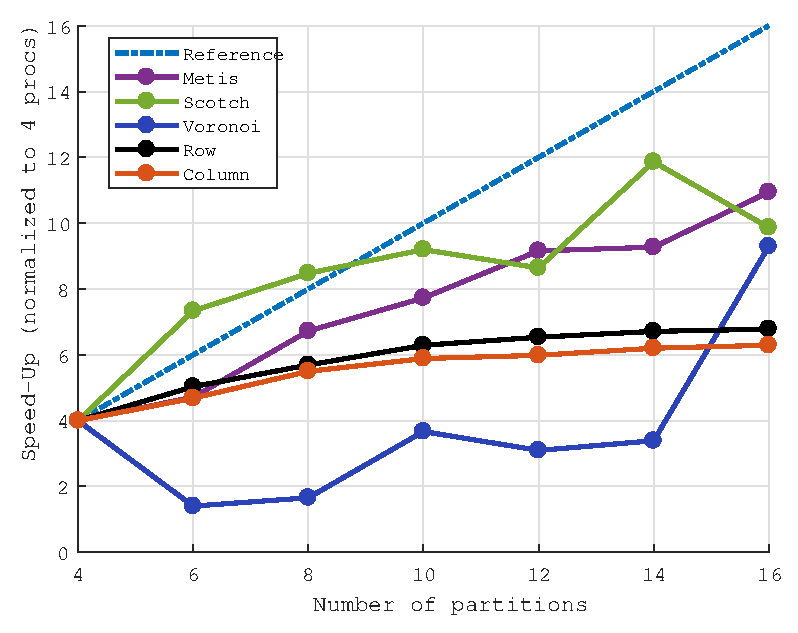
\includegraphics[width=\textwidth]{robin_400x400_5_speedup.eps}
%		\caption{Robin}
	\end{subfigure}
	\hfill
	\begin{subfigure}[t]{0.45\textwidth}
		\centering
		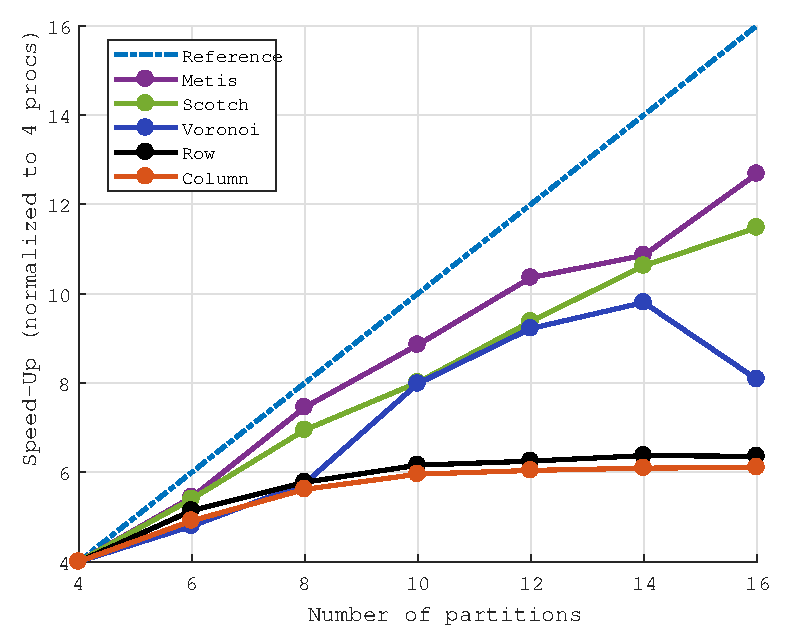
\includegraphics[width=\textwidth]{dirichlet_400x400_5_speedup.eps}
%		\caption{Dirichlet}
	\end{subfigure}
\end{figure}
\vspace*{-8mm}
\begin{figure}[H]\ContinuedFloat
	\begin{subfigure}[t]{0.45\textwidth}
		\centering
		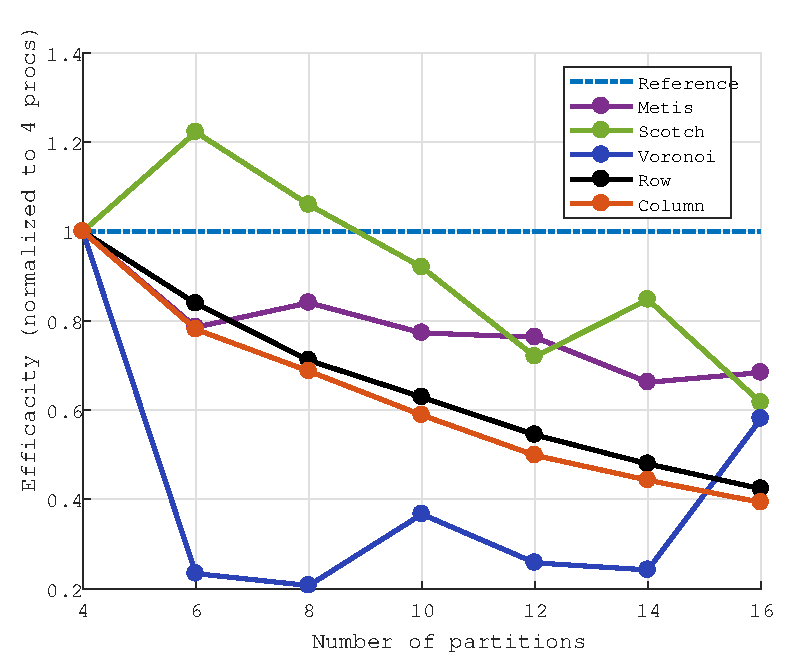
\includegraphics[width=\textwidth]{robin_400x400_5_efficacity.eps}
%		\caption{Robin}
	\end{subfigure}
	\hfill
	\begin{subfigure}[t]{0.45\textwidth}
		\centering
		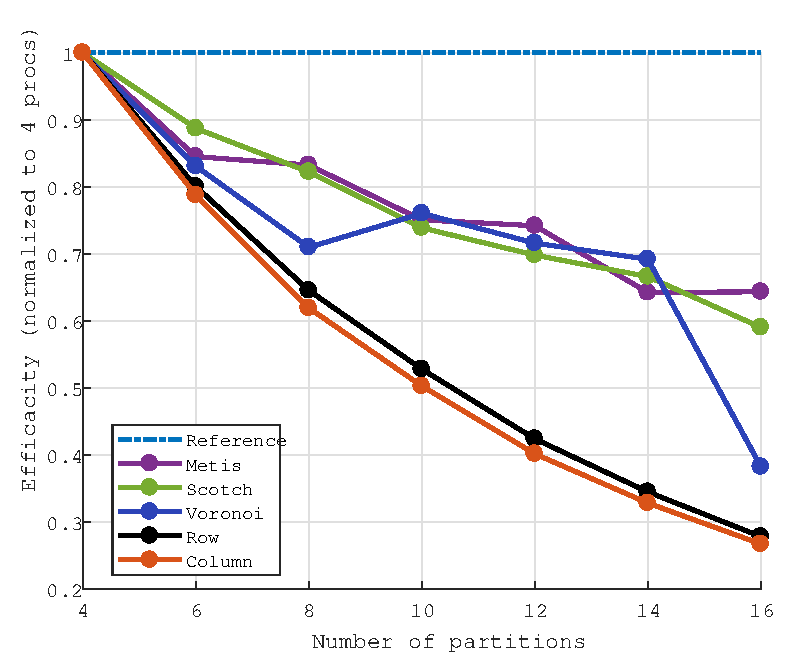
\includegraphics[width=\textwidth]{dirichlet_400x400_10_efficacity.eps}
%		\caption{Dirichlet}
	\end{subfigure}
	\caption{Analyse du cas $400\times400$ avec un recouvrement de taille 5. À droite Robin et à gauche Dirichlet.}
\end{figure}
\noindent Dans ces tests nous avons volontairement omis le partitionnement en damier qui induit des temps de calcul vraiment plus longs comme nous l'avons montré dans la sous-section précédente. Cette partie mets en évidence l'importance de la taille du recouvrement rapportée à la taille totale. Globalement tous les temps de calculs sont augmentés et le nombre d'itérations aussi. Tout le reste est sensiblement pareil que dans l'exemple précédent.

\subsubsection{Résolution $400\times 400$, recouvrement de taille 10}
\begin{figure}[H]
	\centering
	\begin{subfigure}[t]{0.45\textwidth}
		\centering
		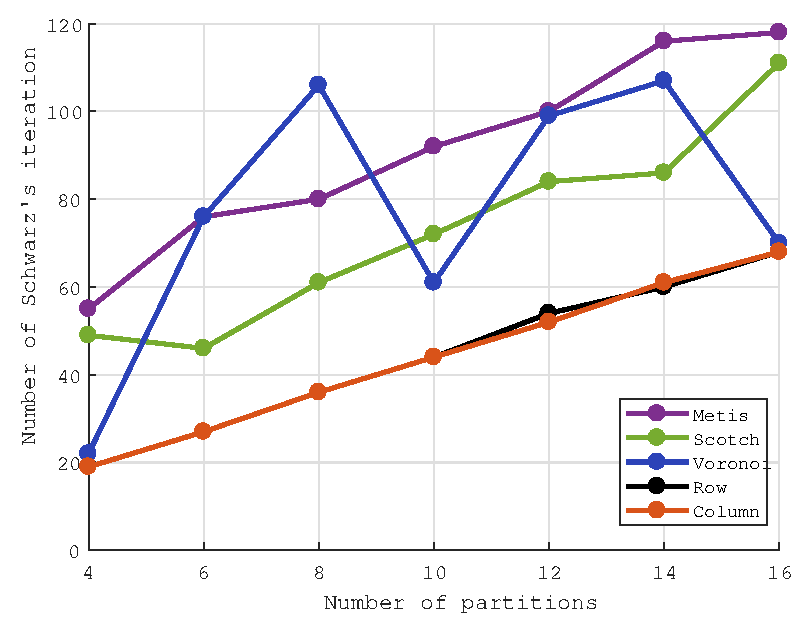
\includegraphics[width=\textwidth]{robin_400x400_10_iter.eps}
%		\caption{Robin}
	\end{subfigure}
	\hfill
	\begin{subfigure}[t]{0.45\textwidth}
		\centering
		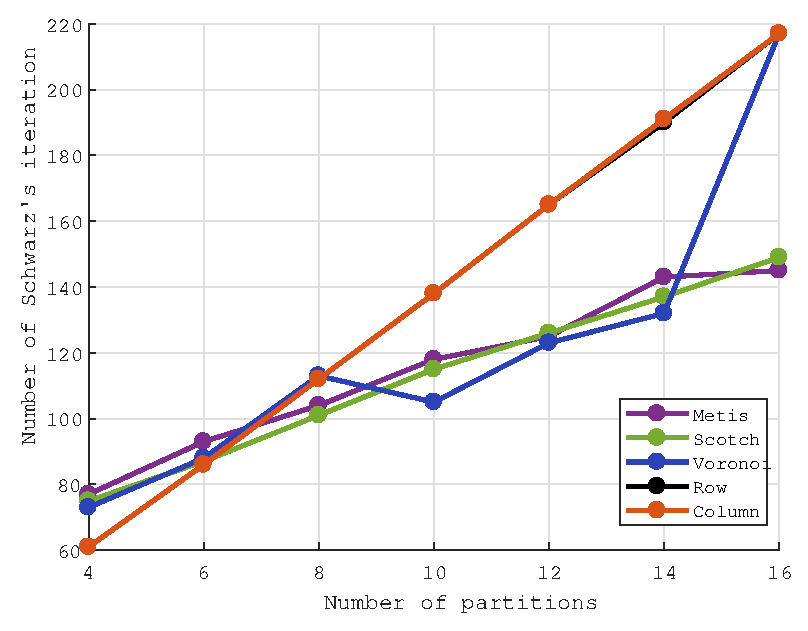
\includegraphics[width=\textwidth]{dirichlet_400x400_10_iter.eps}
%		\caption{Dirichlet}
	\end{subfigure}
\end{figure}
\begin{figure}[H]\ContinuedFloat
	\begin{subfigure}[t]{0.45\textwidth}
		\centering
		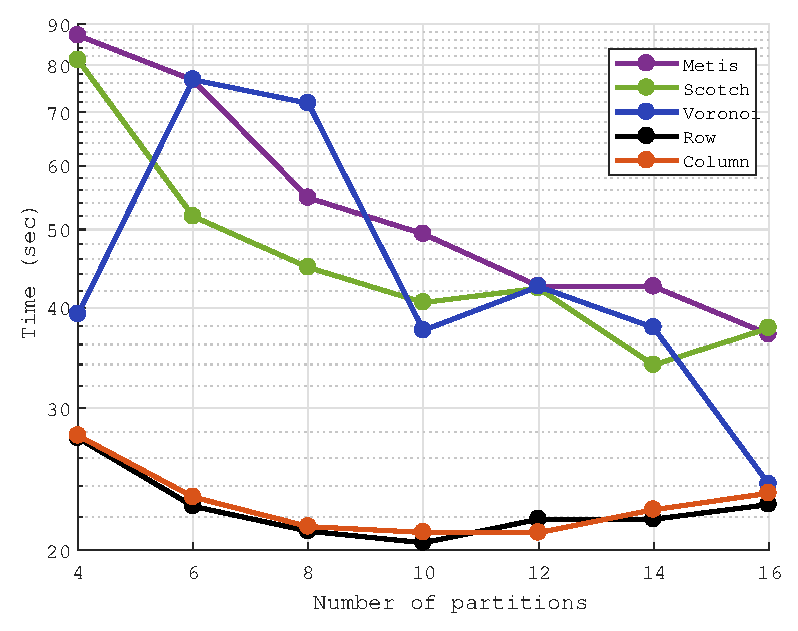
\includegraphics[width=\textwidth]{robin_400x400_10_time.eps}
%		\caption{Robin}
	\end{subfigure}
	\hfill
	\begin{subfigure}[t]{0.45\textwidth}
		\centering
		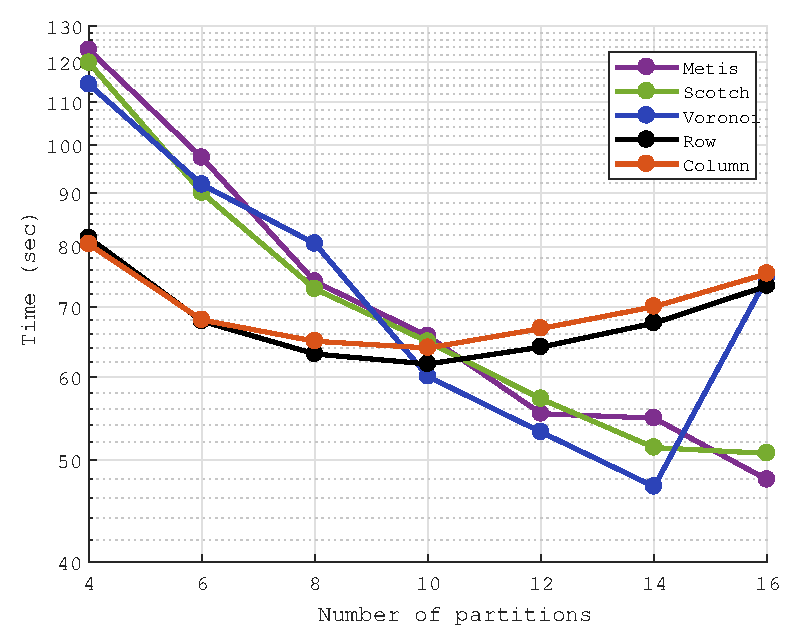
\includegraphics[width=\textwidth]{dirichlet_400x400_10_time.eps}
%		\caption{Dirichlet}
	\end{subfigure}
\end{figure}
\begin{figure}[H]\ContinuedFloat
	\begin{subfigure}[t]{0.45\textwidth}
		\centering
		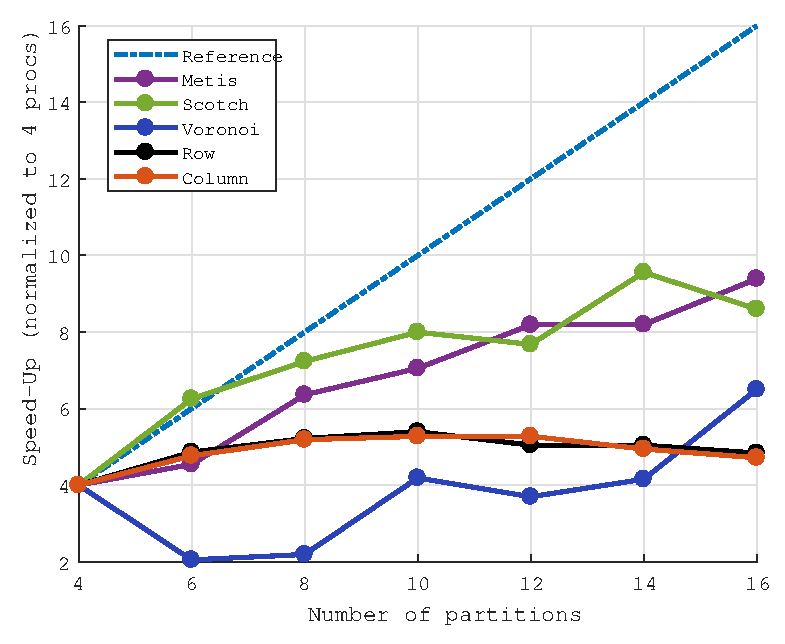
\includegraphics[width=\textwidth]{robin_400x400_10_speedup.eps}
%		\caption{Robin}
	\end{subfigure}
	\hfill
	\begin{subfigure}[t]{0.45\textwidth}
		\centering
		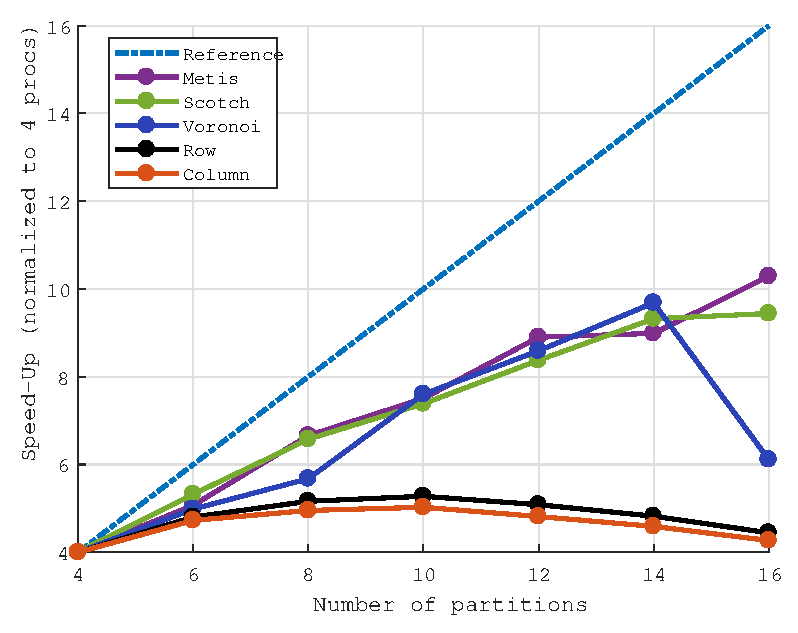
\includegraphics[width=\textwidth]{dirichlet_400x400_10_speedup.eps}
%		\caption{Dirichlet}
	\end{subfigure}
\end{figure}
\begin{figure}[H]\ContinuedFloat
	\begin{subfigure}[t]{0.45\textwidth}
		\centering
		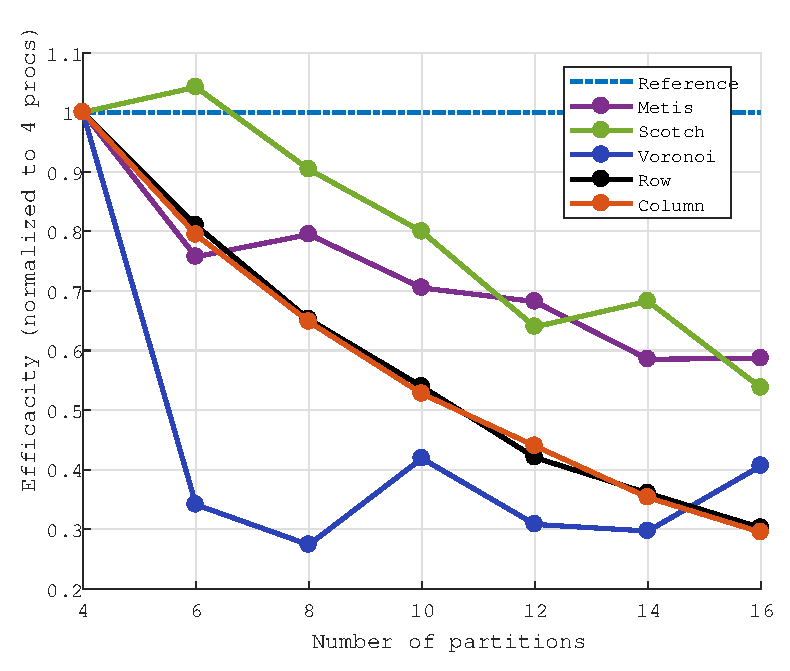
\includegraphics[width=\textwidth]{robin_400x400_10_efficacity.eps}
%		\caption{Robin}
	\end{subfigure}
	\hfill
	\begin{subfigure}[t]{0.45\textwidth}
		\centering
		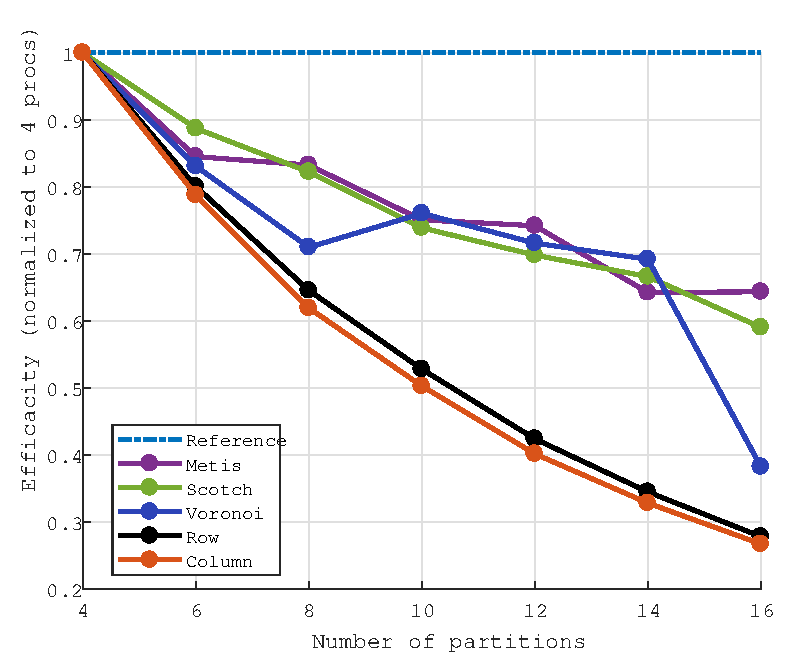
\includegraphics[width=\textwidth]{dirichlet_400x400_10_efficacity.eps}
%		\caption{Dirichlet}
	\end{subfigure}
	\caption{Analyse du cas $400\times400$ avec un recouvrement de taille 10. À droite Robin et à gauche Dirichlet.}
\end{figure}
\noindent Cette partie porte sur la taille du recouvrement, les principales différences à pointer du doigt sont les temps de calculs et le nombre d'itérations nécessaires qui diminuent fortement.

\subsubsection{Erreur et solution numérique : $200\times 200$ - recouvrement $5$ - $4$ partitions avec Metis}
\noindent Nous proposons quelques rendus d'erreur pour le problème \eqref{eq:problem2}. Pour se faire nous avons utilisé un maillage $200\times 200$ partitionné en 4 avec Metis, un recouvrement de taille 5 et des conditions de Robin.
\vspace{-8mm}
\begin{figure}[H]
	\begin{subfigure}[t]{0.45\textwidth}
		\centering
		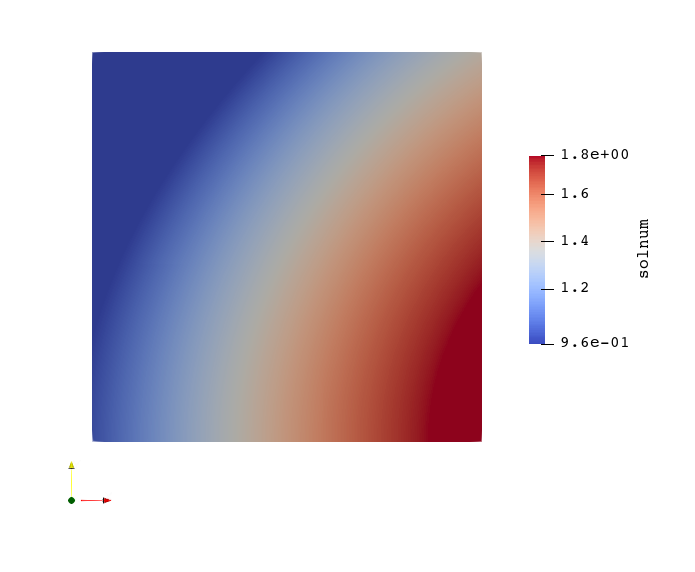
\includegraphics[width=0.95\textwidth]{metis_200_200_solnum.png}
		%		\caption{Robin}
	\end{subfigure}
	\hfill
	\begin{subfigure}[t]{0.45\textwidth}
		\centering
		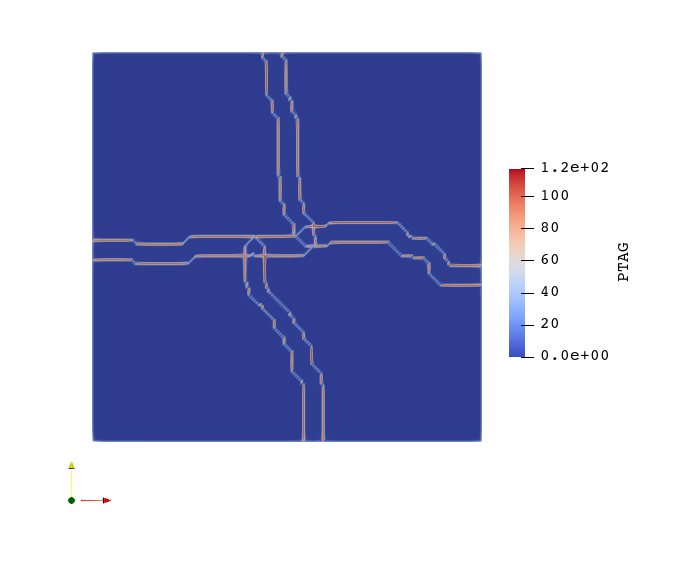
\includegraphics[width=0.95\textwidth]{metis_200_200_ptag.png}
		%		\caption{Dirichlet}
	\end{subfigure}
	\caption{Solution analytique à gauche et tags de partitionnement à droite.}
\end{figure}
\begin{figure}[H]
	\begin{subfigure}[t]{0.45\textwidth}
		\centering
		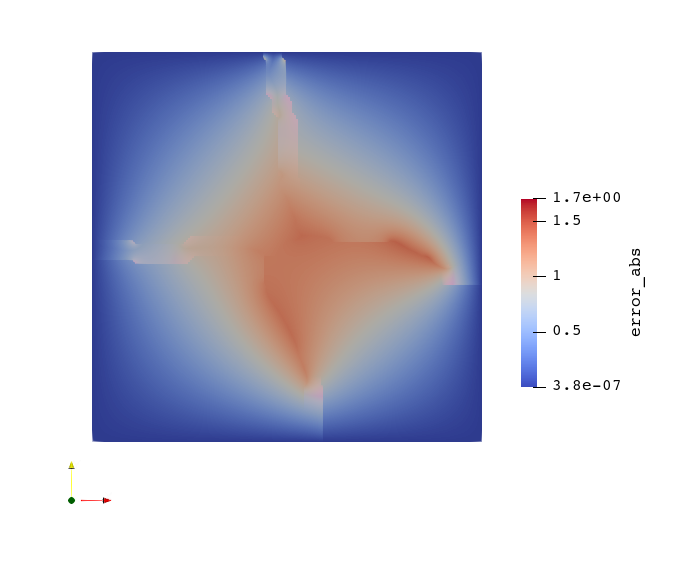
\includegraphics[width=0.95\textwidth]{metis_200_200_0_err.png}
		%		\caption{Robin}
	\end{subfigure}
	\hfill
	\begin{subfigure}[t]{0.45\textwidth}
		\centering
		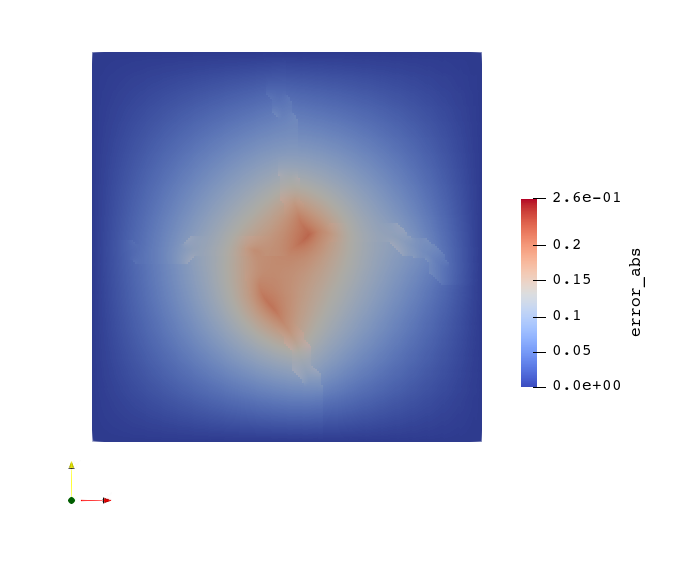
\includegraphics[width=0.95\textwidth]{metis_200_200_10_err.png}
		%		\caption{Dirichlet}
	\end{subfigure}
	\caption{Évolution de l'erreur en valeur absolue point à point aux itérations 1 et 11 sur 37.}
\end{figure}
\begin{figure}[H]
	\centering
	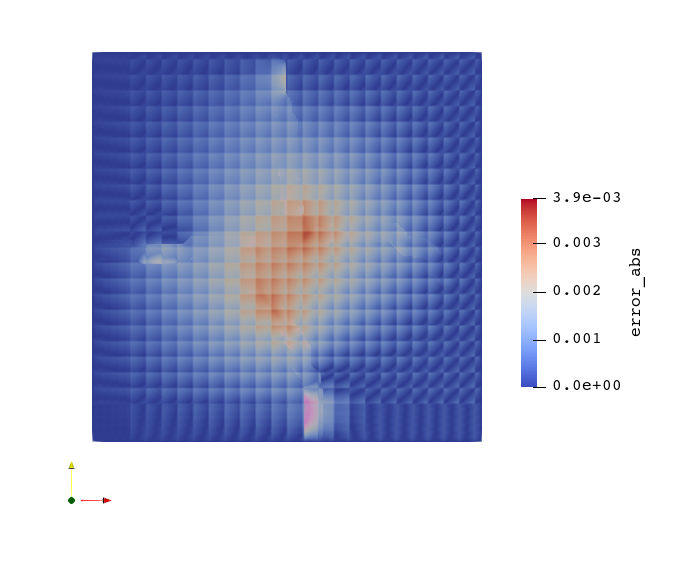
\includegraphics[width=0.6\textwidth]{metis_200_200_30_err.png}
	\caption{Erreur en valeur absolue point à point à l'itération 30 sur 37.}
\end{figure}
\noindent L'erreur décroît bien au cours des itérations de Schwarz, donc la solution numérique converge petit à petit vers la solution analytique. La seule remarque à faire ici est sur le comportement visuel de l'erreur à l'itération 30 sur 37 : une grille semble apparaître et elle ne suit pas le maillage de base et encore moins les partitions. Nous ne sommes pas capable malheureusement d'expliquer le phénomène bien que celui-ci soit présent pour tous les types de partitionnement que nous avons testé. Un début d'explication peut être néanmoins tenté : il se peut que ce soit un comportement inhérent à notre solveur bigradient conjugué stabilisé mais nous n'en savons pas plus.

\subsection{Conclusion}
\noindent Pour conclure cette partie nous mettrons en lumière l'intérêt tout particulier des partitionnements Metis et Scotch. Ils sont un bon compromis selon tous nos tests lorsque que nous les allions à des conditions de Robin, autant du point de vue de la conversion Robin vers Dirichlet, que du temps de calcul ou de l'efficacité.\\
Implémenter la suite de code Lyra nous a permis de réfléchir plus en profondeur sur les différentes méthodes de partitionnement, sur MPI en lui-même et sur l'utilisation de PlaFRIM.\\
Il reste nombre de points à approfondir, notamment l'utilisation de communications non-bloquantes.
\newpage
\listoffigures

%\begin{appendices}
%	\section{Formules de Green}
%	\begin{equation}
%		
%	\end{equation}
%\end{appendices}
\end{document}
